
\chapter{Quality Control of RPCs}
The Resistive Plate Chamber (RPC) is chosen as the sensitive detector
of the ICAL. The ICAL requires approximately 30000 RPCs to function at
its full capacity. The INO~Project is proposed to operate for at-least
for 20 years. All the RPCs thus must operate without showing any
significant ageing during the period of operation. Hence, various
tests are performed during and after production of the RPCs.
\begin{figure}[h]
  \centering
  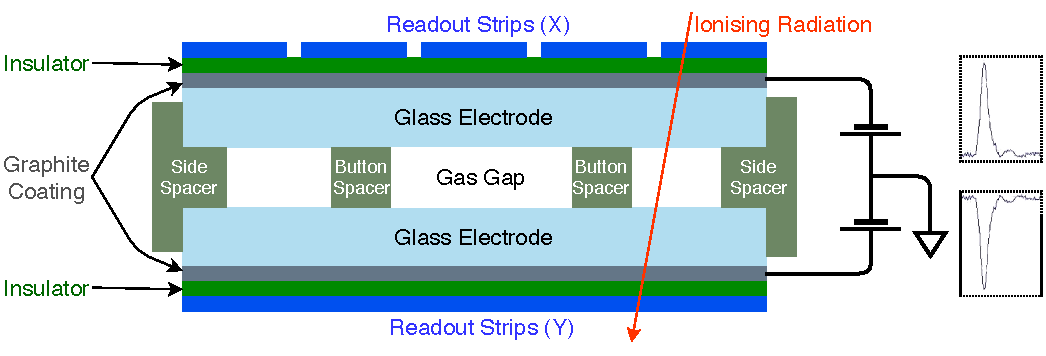
\includegraphics[width=0.9\textwidth]{basic_rpc.pdf}
  \caption{Schematic of a Resistive Plate Chamber.}
  \label{fig:rpc}
\end{figure}

The RPCs that are going to be used in the ICAL are made of glass.
The two glass plates, kept at a uniform distance of 2\,mm using the
help of poly-carbonate buttons, are sealed from four sides to create
a leak-tight gas-gap. Both of the outer sides of the gap are coated
with semi-resistive graphite paint to form the electrodes where the
high voltages can be applied. A mixture of gas is then flown inside
the gap via strategically placed nozzles. In the ICAL, the gas
mixture is composed of R134a\,(95.2\%), iso-C$_4$H$_{10}$\,(4.5\%) and
SF$_6$\,(0.3\%).\footnote{R134a is a commercial name of
  1,1,1,2-Tetrafluoroethane.}
The R134a acts as the target medium for the incident particles.
The electrons emitted in the ionisation process initiated by the
passing particles create an avalanche under the influence of
the applied electric field. The induced signal of the avalanche is
then detected by two copper pickup panels on both sides of the gap.
The iso-C$_4$H$_{10}$ act as a photon-quencher which absorbs
the emitted photons in the recombination process limiting the
formation of secondary avalanches. On the other hand, the SF$_6$ being
an electro-negative gas acts as an electron-quencher which localises
the signal within a small area yielding better position resolution.

During the up-time of the ICAL detector, more than 200000\,litres of
the gas mixture will be circulating inside the 30000 RPCs.
A closed-loop gas circulating system (CLS) is designed for this
purpose whose main aim is to recirculate the gas mixture, minimising
the wastage of gas.
The CLS and the plumbings operate at much higher pressure than the
atmosphere, but the RPCs are proposed to be operated at an excess
pressure of just 10\,mmWC above atmospheric pressure. Thus the RPCs
pose an additional challenge of keeping the CLS free of contamination
because of this little pressure barrier.
The leakage of outside atmosphere into the
system will introduce water vapour and oxygen inside the RPCs which
can increase the risk of damaging the RPCs\cite{rpc_c,rpc_w}.
The fluorine present in the RPC gas mixture can produce hydrofluoric
after reacting with the water vapour during the avalanche.
The hydrofluoric acid which is corrosive to glass can damage the
inside surface of the gas gaps. On the other hand, the oxygen being
an electro-negative in nature can affect the performance of the
detector. Due to these reasons, a proper leak test is required to be
performed on all the glass gaps during the production as~well~as the
time of operation. Moreover, the impurities in the
CLS also needed to be monitored during the operation of ICAL.

\section{Leak Test of RPCs}
To estimate the leakage, the RPC is first pressurised up-to 45\,mmWC
above the atmospheric pressure and then sealed.\footnote{Millimetres
  water column, abbreviated to mmH$_2$O or mmWC, is a unit of pressure.
  It is the pressure required to support a water column of the
  specified height. 1\,mmWC\,$\simeq$\,0.098\,mbar.}
The pressure inside the RPC is monitored over a long period.
The schematics of a typical leak test setup is shown in the
Figure~\ref{fig:test_rpc}. 
\begin{figure}
  \centering
  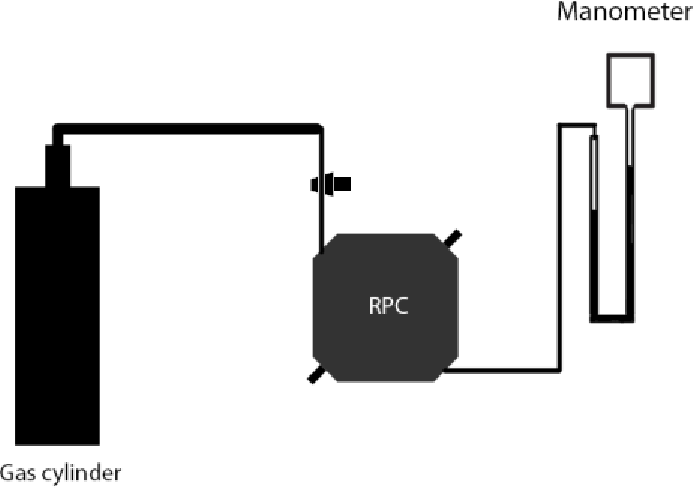
\includegraphics[width=0.6\textwidth]{test_rpc.pdf}
  \caption{Schematics of a typical leak test setup.}
  \label{fig:test_rpc}
\end{figure}
A conventional choice of the sensor to monitor the pressure inside
the RPC is the manometer setup as shown in Figure~\ref{fig:test_rpc}.
Now, the limitation of leak rate estimation using the manometer comes
from its observable quantity. The manometer measures the difference
between two pressures $\left(\Delta P\right)$, the atmospheric
pressure $\left(P_{\mathrm{rpc}}\right)$ and the RPC pressure
$\left(P_{\mathrm{atm}}\right)$, which can be widely affected by the
change of the atmospheric pressure, the room temperature and the
volume of the chamber. Hence, the estimation of leak rate using a
manometer is only valid in two scenarios, (i) if the atmospheric
pressure, the room temperature and the volume of the chamber are
kept constant and/or (ii) if the leak rate is very large.

But both the atmospheric pressure and room temperature are constantly
affected by the solar atmospheric tides and changes in weather.
\footnote{The solar atmospheric tides are generated by the periodic
  heating of the atmosphere by the Sun. This regular diurnal cycle in
  heating generates tides in the atmosphere that have periods related
  to the solar day.}
In the following, it will be established that the volume of the RPC
gaps also changes with the variation of the ambient pressure and
temperature. Moreover, if the leak from the RPCs is very small then it
is nearly impossible to detect.

Hence, a different leak test method along with the test setup is
developed to overcome the aforesaid limitations. The setup and
technique discussed in the following not only helps to determine
whether the RPC is leaking but also allows to estimate the
magnitude of the leakage. As the number of the RPCs needed to be tested
is large, the setup is required to be simple, portable and
cost-effective. The method is also able to test multiple RPCs
simultaneously without moving them out of the storage area, which thus
limits the possibility of damage to the fragile large glass gaps.

\subsection{Defining the Leak Rate of RPCs}
As per the Poiseuille's law\cite{poiseuille}, the laminar flow rate of a fluid
through a leak path is given in the equation \ref{eq:poiseuille1}.
\begin{equation}
\left(\text{Flow Rate}\right)=\left(\text{Leak Constant}\right)\times\left(\text{Effective Pressure Difference}\right)\label{eq:poiseuille1}
\end{equation}
where, the \textit{Leak Constant} depends on the path of leakage (i.e. crack,
hole, etc) and the viscosity of the gas mixture. The \textit{Leak Constant}
quantifies the leakage in the system. The setup and techniques to calculate
the \textit{Leak Constant}s for the gas gaps are discussed in the following.

Assuming that the leakage from an RPC is very small, it allows the flow of gas
through the leak path to be considered as laminar flow. Also, the variation of
ambient pressure and temperature does not affect the viscosity of the gas
significantly. The equation~\ref{eq:poiseuille1} thus can be used for the case
of RPCs.

\subsection{Experimental Setups}
The schematics of the `standalone' leak-test setup is shown in the
Figure~\ref{fig:schematics}. 
\begin{figure}
  \centering
  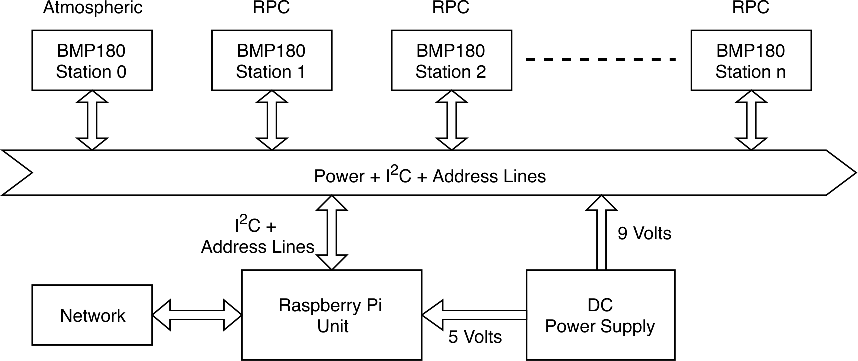
\includegraphics[width=0.9\textwidth]{leaktest_setup.pdf}
  \caption{Schematics of the `standalone' leak test setup.}
  \label{fig:schematics}
\end{figure}
In this setup, instead of measuring the differential pressure using the
conventional manometer, the absolute pressure and temperature inside and
outside of the gas gap are measured using the sensor module, BMP180
manufactured by BOSCH\cite{bmp180}. The BMP180 is a piezo-resistive sensor
having an accuracy of 0.7\,mmWC and 0.05\,$^{\circ}$C in the measurement of
pressure and temperature respectively. This sensor is capable of recording
data samples for the minimum time interval of 76\,ms. The leak test module is
shown in the Figure~\ref{fig:setup}(\subref{fig:pc3}). 
\begin{figure}
  \centering
  \begin{subfigure}[b]{0.34\textwidth}
    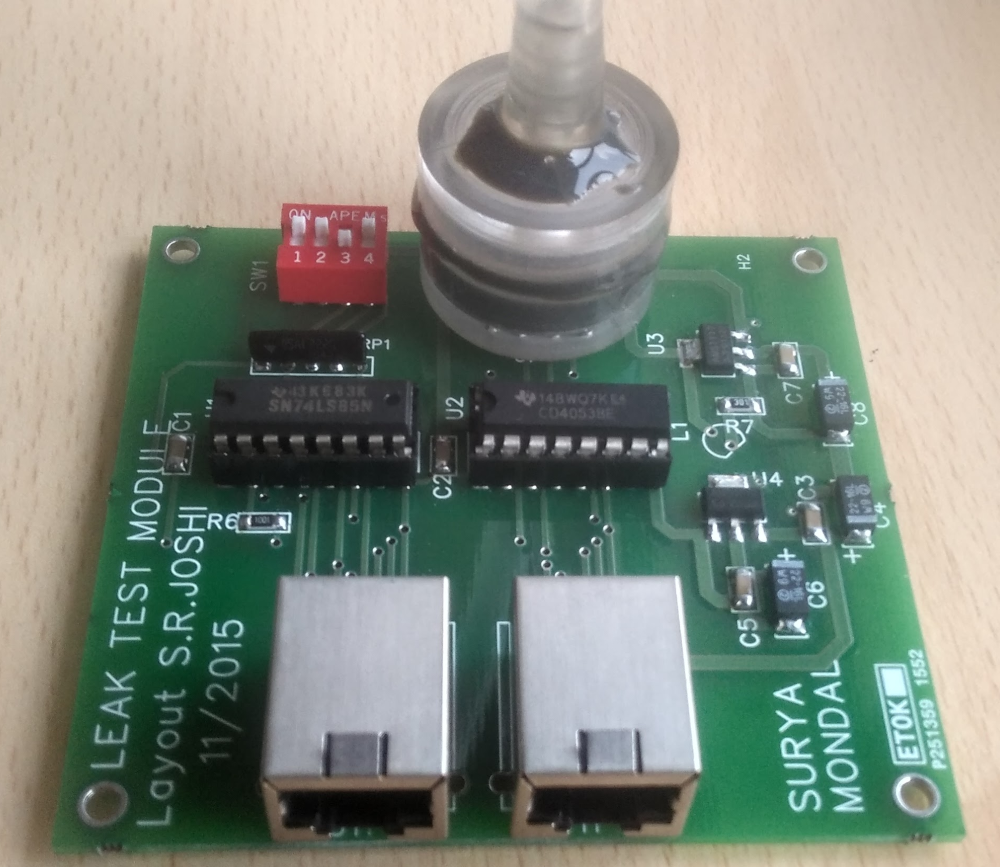
\includegraphics[width=\textwidth]{pc3.png}
    \caption{Leak Test Module.}
    \label{fig:pc3}
  \end{subfigure}
  \begin{subfigure}[b]{0.64\textwidth}
    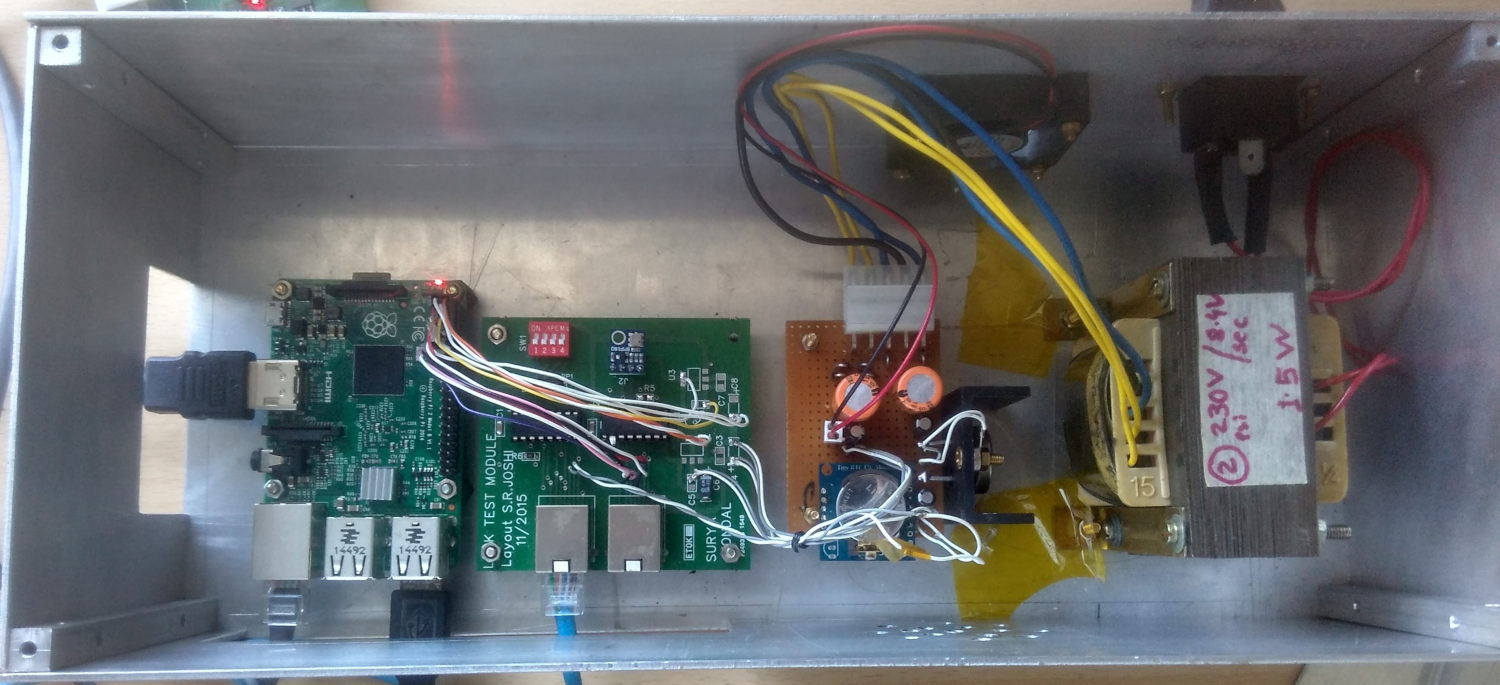
\includegraphics[width=\textwidth]{pc2.png}
    \caption{Raspberry Pi B \& Power Supply Module.}
    \label{fig:pc2}
  \end{subfigure}
  \caption{Leak Test Setup.}
  \label{fig:setup}
\end{figure}
Each of such modules will record the pressure and temperature for one gas gap.
The pressure and temperature data recorded by the module is readout using a
\textit{Raspberry Pi\,v2\,B} (Pi) unit\cite{rpi} shown in the
Figure~\ref{fig:setup}(\subref{fig:pc2}). The data is stored on the on-board
memory of the Pi unit. As shown in Figure~\ref{fig:setup}(\subref{fig:pc3}),
each module has two bus ports. This allows to daisy-chain several leak test
modules and can be controlled from a single Pi unit.

The common bus mainly consists of Power, Data and Address lines. To avoid the
voltage drop in the supply line over a long distance, 9\,V DC is supplied from
the Pi End and converted to the required voltage at each test module. A 4-bit
DIP switch is used on each module to set a unique address for itself. The Pi
acquires the data from each station by selecting its unique address. So, only
one test module is allowed to communicate with the control unit at a time.
As 4-bit address lines are used in this setup, a maximum of fifteen gas gaps
can be tested simultaneously. The system is scalable to handle more gas gaps
simultaneously, by simply adding more address lines. One of the leak test
modules are dedicated to record the ambient pressure and temperature for the
test duration.

The data from the BMP180s can also be acquired without wires by
microcontrollers equipped with WiFi modules (i.e. NodeMCU
module\cite{nodemcu2015}), eliminating the need of the wired common bus and
Pi Unit. One such setup is shown in Figure~\ref{fig:leakwifi}. 
\begin{figure}
  \centering
  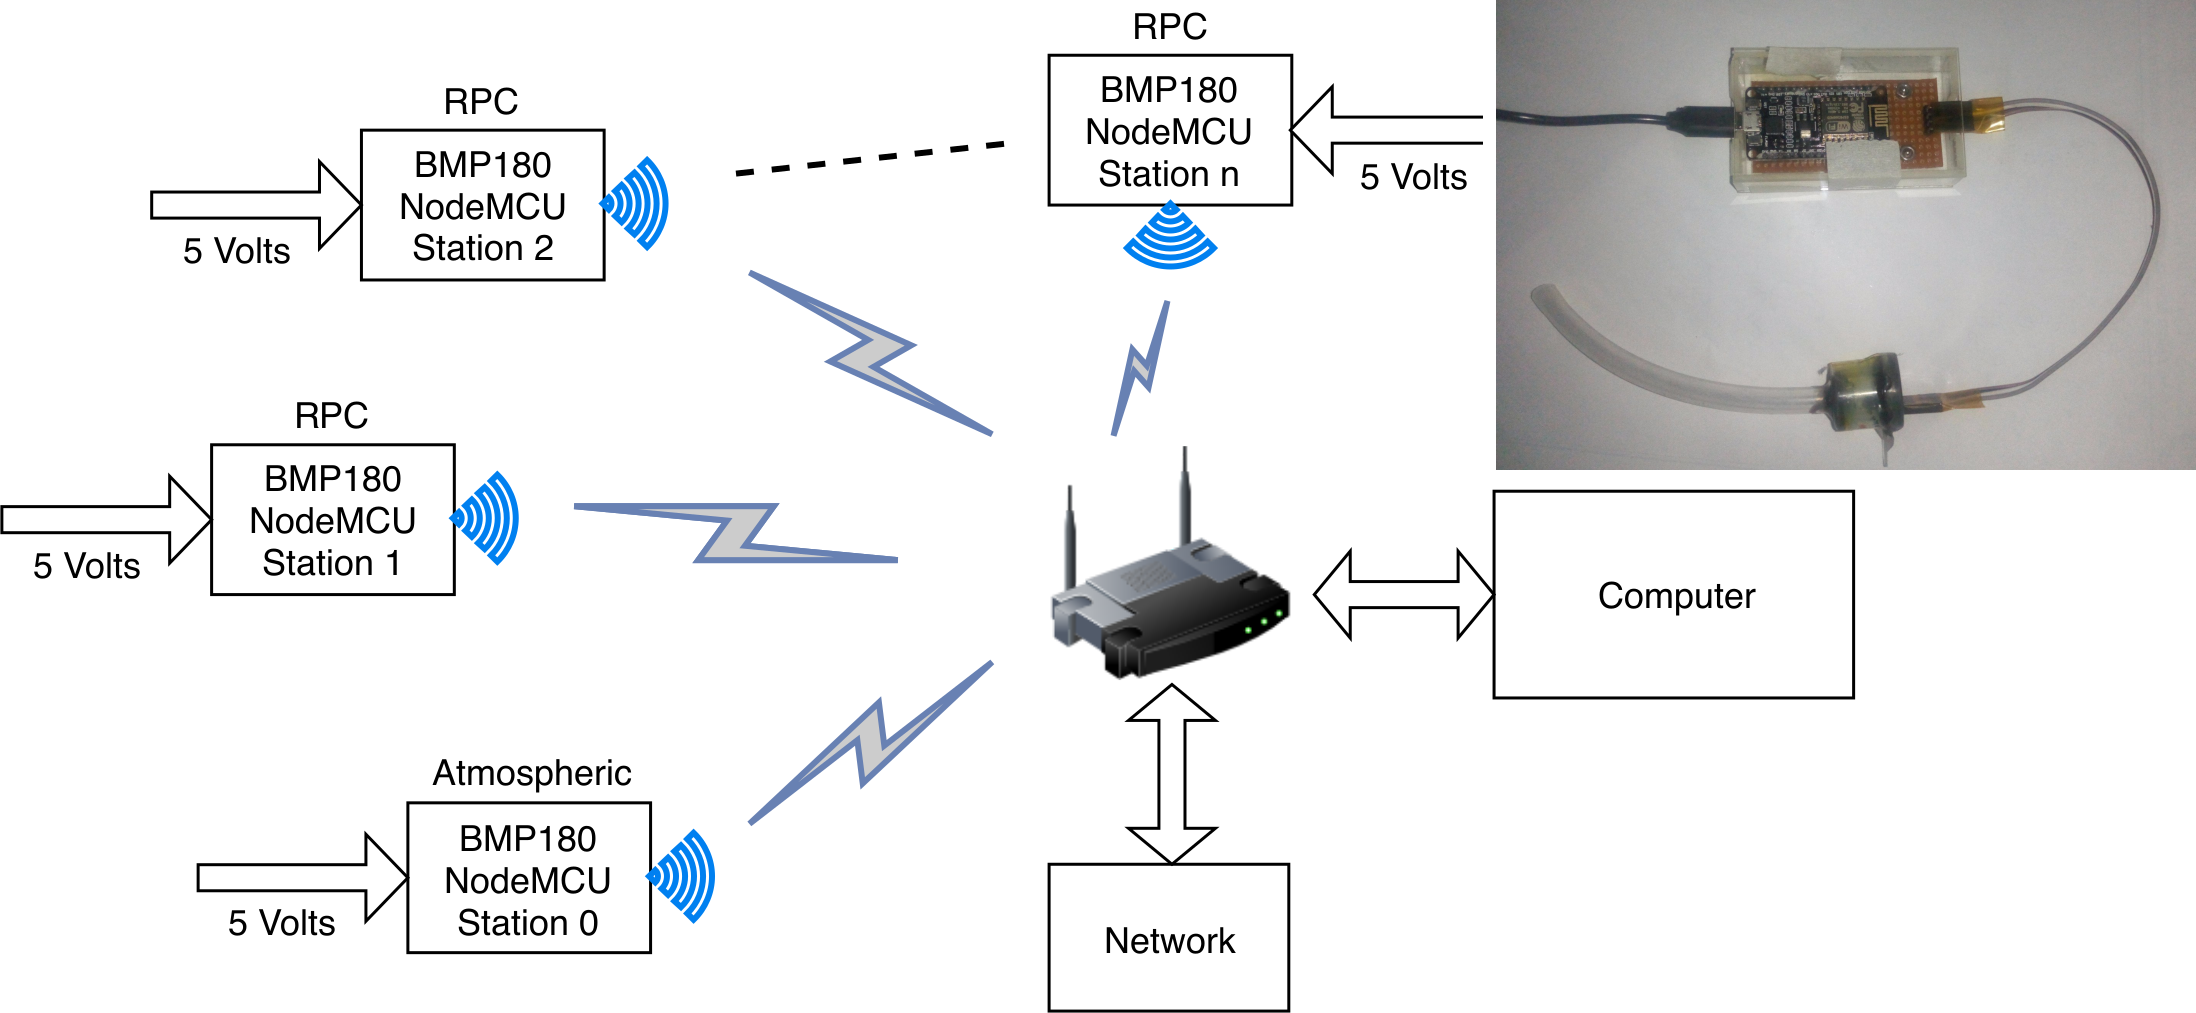
\includegraphics[width=0.99\textwidth]{leaktest_setup_wifi_all.png}
  \caption{Schematics of the WiFi-based leak test setup and one of the
    test-modules (in the inset).}
  \label{fig:leakwifi}
\end{figure}
This setup requires an operational WiFi network at the premises to send the
data to a computer on the same network. If the network is connected to the
internet, then the data can be stored at any remote location also. The
test-modules, being low-power devices, can also be powered with small
power~banks which makes it hugely advantageous while being used at large
warehouses. Also, the elimination of the long wires makes this setup immune
to electromagnetic interference from other sources. Though this setup is not
`standalone', it is truly scalable which can handle any number of RPC gaps
being tested without changing any of the basic design elements.

In the current setup, the pressure and temperature data from each
sensor along with the atmospheric pressure and temperature data are
recorded continuously with a specified interval of $3$\,seconds.
The final data recorded for a gas gap include the values of the
ambient pressure and temperature, the gas gap pressure and temperature
and the time stamp for each measurement.
The method to quantify the leakage using these data is discussed in the
section~\ref{sec:calculation}.

\subsection{Detection of Button Pop-Ups}\label{sec:button}
The structural stability of the RPC is maintained by the polycarbonate
buttons. However, it is observed that sometimes the glue which is used
to attach the buttons to the glass plates, fails to hold under
pressure which results in detaching of the buttons from the glass
plates.\footnote{Hereafter such an event is referred to as
  `button pop-up'.}
This weakens the structure of RPC. Also during detector operations,
this will increase the spacing between the glass plates, thus
decreasing the effective electric field resulting in reduced signal
strength. Also, for any working RPC, the glue used to attach the
buttons to the glass plates must continue to hold under pressure.
For any RPC gas gap, even if only one button is not attached, that
glass gap will not be suitable to hold more pressure as eventually the
glue for more and more buttons will give away, making the gas gap
weaker. Hence, it is essential to detect any `button pop-up' events
during the leak test.

With each `button pop-up' event, the volume of the RPC gap increases which in turn
results in a decrease in the pressure inside the gap. Thus the pressure
difference between the outside and inside of the gap decreases. In the plot of
pressure difference with time, this effect will be observed as a sudden drop
in the pressure difference. The Figure~\ref{fig:button} shows the variation of
pressure difference with time for an RPC where there are `button pop-up'
events. 
\begin{figure}
  \centering
  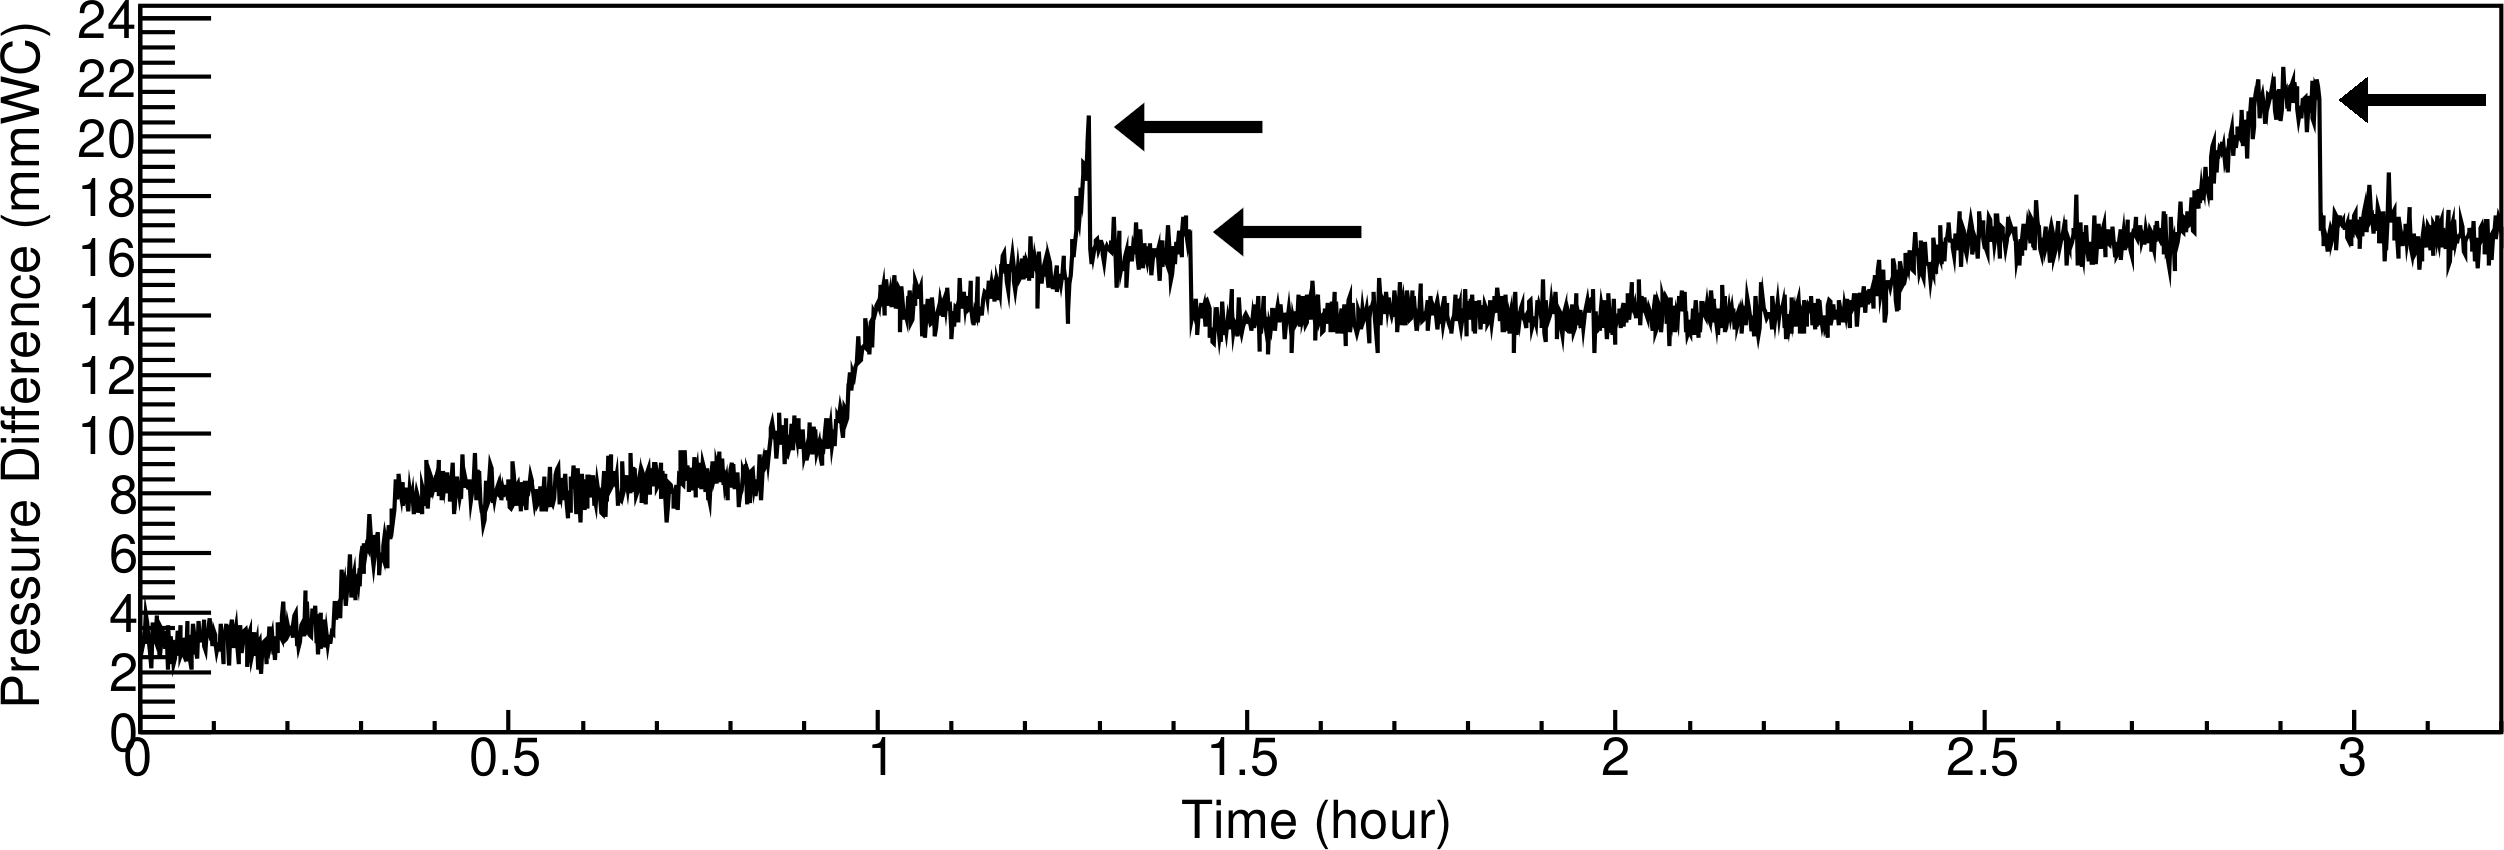
\includegraphics[width=0.99\textwidth]{button.png}
  \caption{Variation of pressure difference with time showing button pop-ups.}
  \label{fig:button}
\end{figure}
It can be observed in the figure that there are three `button pop-up'
events (pointed by arrows) in this RPC and also seen that these
`button pop-up' events result in a decrease in the pressure difference
within a very short time. These events cannot be detected with
conventional manometers unless the pressure is recorded continuously
using a precise differential pressure sensor. Hence, the apparatus,
described in the current paper, is very helpful in detecting the
`button pop-up' events during the test.

It is also to be noted that the method to quantify the leakage
discussed in the following, fails if the data includes button-pop
event(s) in it.

\subsection{Leak Rate Calculation}\label{sec:calculation}
The variation of temperature of the gas gap and variation of pressure in the
gas gap as well as atmosphere respectively with time are illustrated in the
Figure \ref{fig:temp}(a) and \ref{fig:temp}(b). 
\begin{figure}[h]
  \centering
  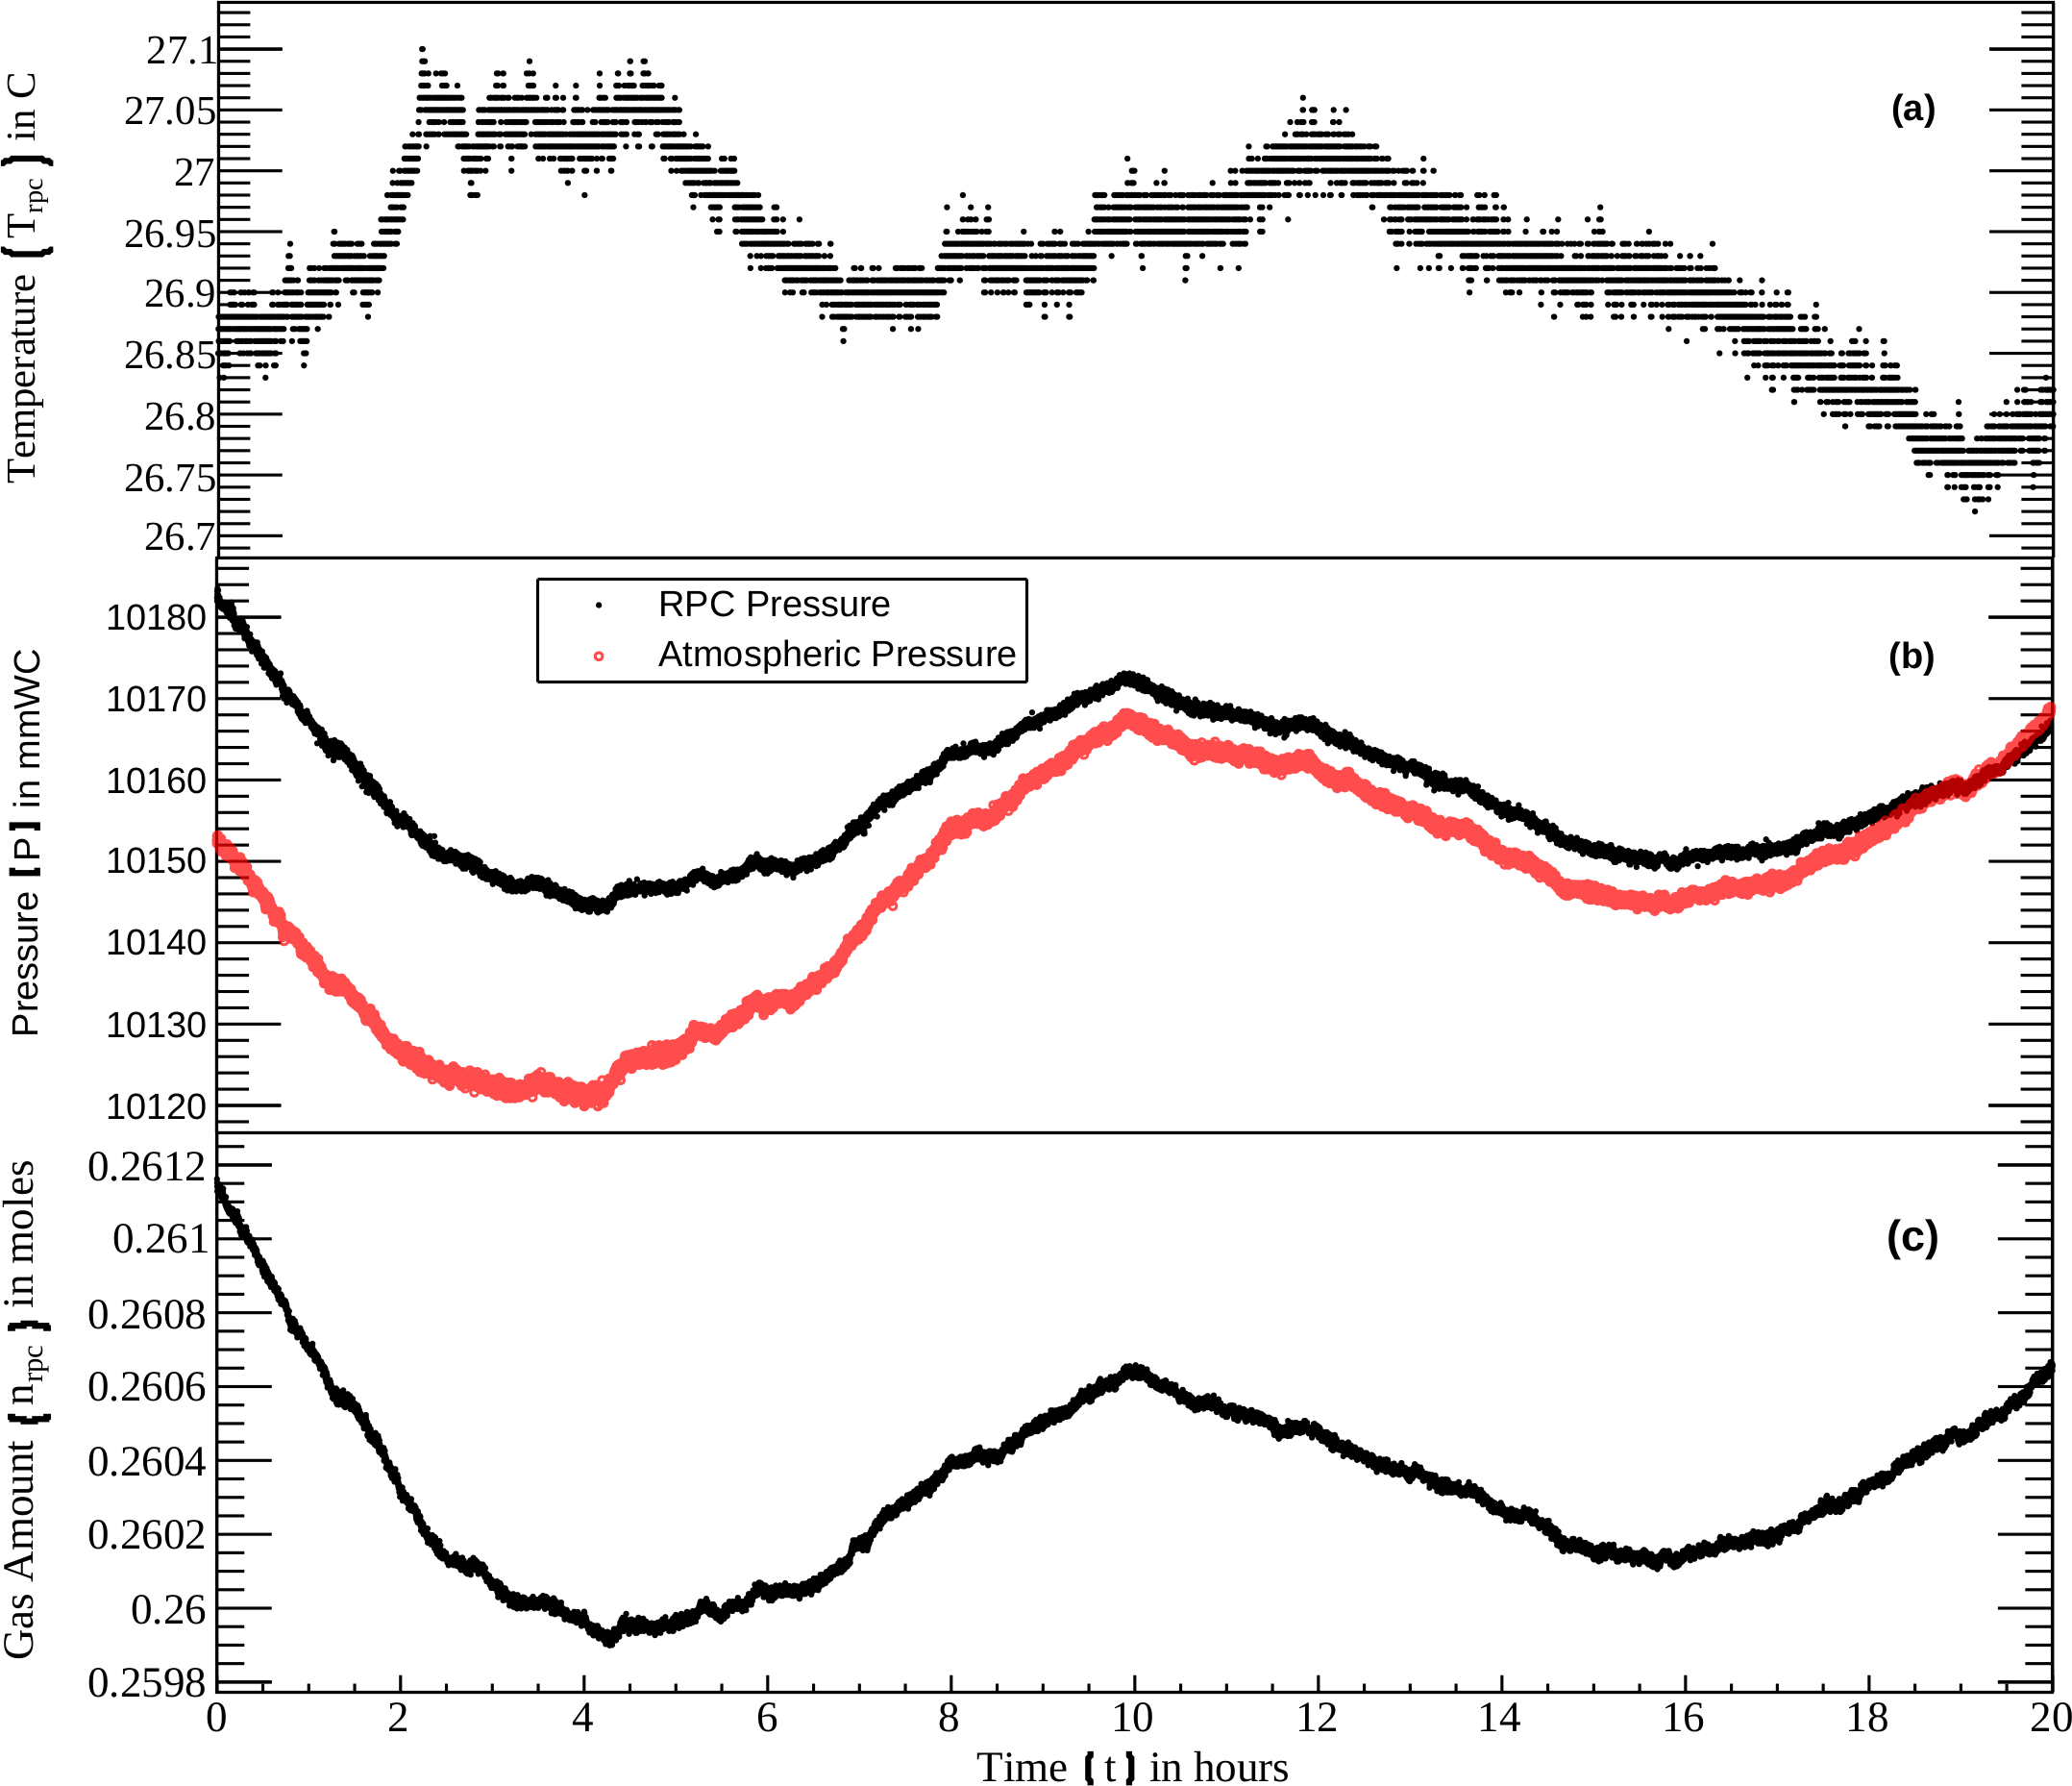
\includegraphics[width=0.99\textwidth]{all_57_gen.png}
  \caption{\textbf{(a)} Variation of temperature $\left(T_{\textrm{rpc}}\right)$
    with time, \textbf{(b)} Variation of atmospheric
    $\left(P_{\textrm{atm}}\text{ : Black}\right)$ and RPC
    $\left(P_{\textrm{rpc}}\text{ : Red}\right)$ pressure with time, \textbf{(c)}
    Amount of gas in the RPC with time assuming $V_{\textrm{rpc}}=6.3$\,litres
    for sample RPC gap-1.}
  \label{fig:temp}
\end{figure}
The periodic variation of the atmospheric pressure shown in the
Figure~\ref{fig:temp}(b) is called the Solar Atmospheric Tide. It can be
observed that the pressure inside the gap is following the trend of atmospheric
pressure. This implies that the volume of the gap changes with the change of
atmospheric pressure. The change in room temperature also affects the pressure
inside the RPC, again affecting the volume of the RPC gap. This change of the
volume during the leak test poses the main difficulty in calculating the leak
rate.

Now, from the Ideal Gas Law, the amount of gas ($n$), inside a chamber of
volume $V$, can be calculated at time $t$ using the following equation,\footnote{All the values of $P$, $V$ and $T$ are converted suitably to calculate the value of $n$ in mole.}
\begin{equation}
  n_{\textrm{rpc}\mid t}=\frac{P_{\textrm{rpc}\mid t}V_{\textrm{rpc}\mid t}}{RT_{\textrm{rpc}\mid t}} \label{mole}
\end{equation}
where, $R$ is the ideal gas constant having the value
8.314\,J\,mole$^{-1}$\,K$^{-1}$. From the dimensions of the gas gap,
the volume of the RPC is estimated to approximately 6.3\,litres.
Taking this into consideration, the amount of gas inside the gap can
be calculated using the equation~\ref{mole}.
The Figure~\ref{fig:temp}(c) shows the apparent variation
of the amount of gas within the gap with respect to time.
The instantaneous leak rate of a gap can be quantified as the slope
of this plot at any particular instant.

To estimate the absolute leak rate, Poiseuille's equation for compressible
fluids\cite{poiseuille} is used. The Poiseuille's equation of Leak Rate at time
$t$ for compressible fluids is given in the equation \ref{eq:poiseuille},
\begin{equation}
  \underbrace{\left.\frac{\mathrm{d}n_{\textrm{rpc}}}{\mathrm{d}t}\right| _t}_\text{flow/leak rate}=\underbrace{\textrm{C}_{\textrm{Leak}}}_\text{flow/leak constant}\times\underbrace{\left(\frac {P_{{\textrm{rpc}\mid t} }^{2}-P_{{\textrm{atm}\mid t} }^{2}}{2P_{{\textrm{rpc}\mid t} }}\right)}_\text{effective pressure difference}\label{eq:poiseuille}
\end{equation}
where, $\textrm{C}_{\textrm{Leak}}$ depends on the path of leakage (i.e. crack,
hole, etc) and the viscosity of the gas mixture and it quantifies the leakage
in the system.\footnote{The viscosity of the gas is assumed to be constant over
  the small changes of room temperature during the test period. In case of
  large changes in temperature, the changes in the value of viscosity are also
  needed to be considered.} The Figure~\ref{fig:preQt} shows the leak rate
$\left(\frac{\mathrm{d}n_{\textrm{rpc}}}{\mathrm{d}t}\right)$ which is calculated
from Figure~\ref{fig:temp}(c) as a function of the effective pressure
difference $\left(\frac{P_{\textrm{rpc}}^{2}-P_{\textrm{atm}}^{2}}{2P_{\textrm{rpc}}}\right)$.\footnote{It is assumed that mole\,$\simeq$\,22.4\,litres for better visualisation.} 
\begin{figure}
  \centering
  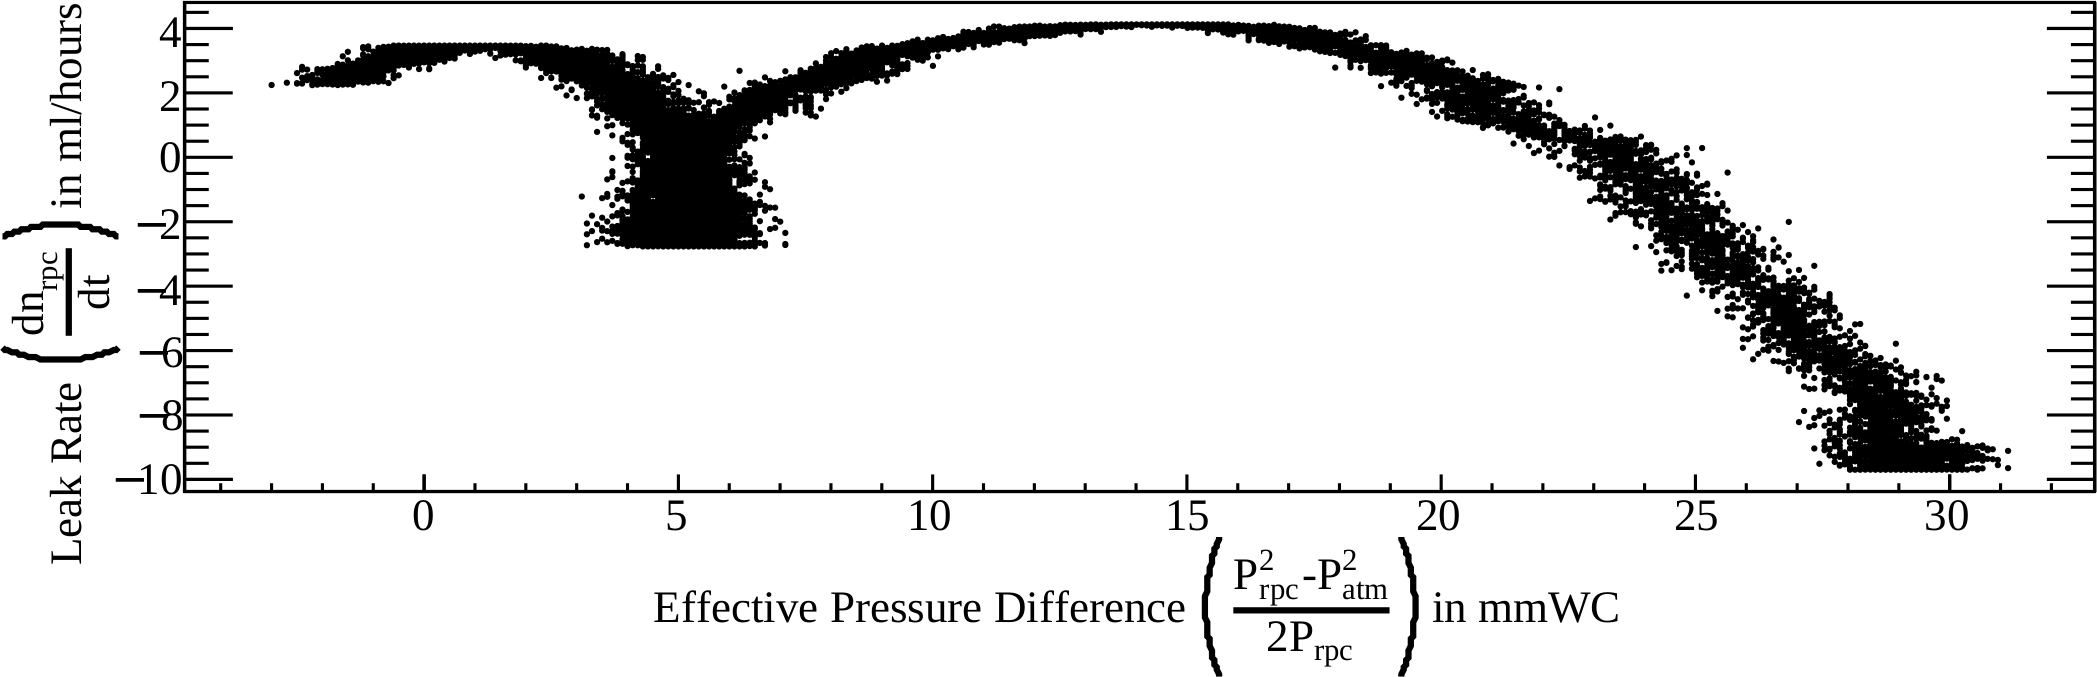
\includegraphics[width=0.99\textwidth]{Q_dP_57_pre.png}
  \caption{$\frac{\mathrm{d}n_{\textrm{rpc}}}{\mathrm{d}t}$ vs
    $\frac{P_{\textrm{rpc}}^{2}-P_{\textrm{atm}}^{2}}{2P_{\textrm{rpc}}}$ for the sample
    RPC gap-1 without any correction.}
  \label{fig:preQt}
\end{figure}

According to the equation~\ref{eq:poiseuille}, it is expected to behave like a
straight line passing through the origin with the slope
$\left(\textrm{C}_{\textrm{Leak}}\right)$ quantifying the leakage in the system
but the observed distribution is not a straight line. Also, the gas gap under
test is sealed from the inlet. Hence, no more gas is getting filled but the
Figure~\ref{fig:temp}(c) shows an apparent increase in the amount of gas inside
the gap. This discrepancy is appearing as the change in the volume of the RPC
is not accounted for in the calculation. Now, as the change in the volume of the
RPC gap cannot be measured directly during the test period, a different
approach is adopted.

To compensate for this change in volume, the volume of the RPC gap at time $t$
is represented by the equation~\ref{vcterm},
\begin{equation}
  V_{\textrm{rpc}\mid t} = \underbrace{V_{\textrm{rpc}}}_{\text{Approx. Volume}}\times\underbrace{\left(1-x_T\left(T_{\textrm{rpc}\mid t}-T_{\textrm{rpc}\mid t=0}\right)\right)}_{\text{Correction for Temperature Change}}\times\underbrace{\left(1-x_P\left(P_{\textrm{atm}\mid t}-P_{\textrm{atm}\mid t=0}\right)\right)}_{\text{Correction for Pressure Change}}\label{vcterm}
\end{equation}
where, $T_{\textrm{rpc}\mid t=0}$ and $P_{\textrm{atm}\mid t=0}$ are equal to
$T_{\textrm{rpc}}$ and $P_{\textrm{atm}}$ at time\,$t=0$, respectively.\footnote{Suffix `atm' denotes the measurements acquired from atmosphere.}
Assuming that the change in volume is linear in both the atmospheric pressure
and the room temperature, two independent linear correction terms ($x_P$ and
$x_T$) are introduced.\footnote{Present method of estimation of leak cannot handle change in volume caused by `button pop-up' event during the period of leak test.}
Using the equation~\ref{vcterm} in the equation~\ref{mole}, the $n_{\textrm{rpc}}$
is represented in the equation~\ref{eq:ct}.
\begin{equation}
  n_{\textrm{rpc}\mid t}=\left(\frac{V_{\textrm{rpc}}}{R}\right)\left(\frac{P_{\textrm{rpc}\mid t}}{T_{\textrm{rpc}\mid t}}\right)\left(1-x_T\left(T_{\textrm{rpc}\mid t}-T_{\textrm{rpc}\mid t=0}\right)\right)\left(1-x_P\left(P_{\textrm{atm}\mid t}-P_{\textrm{atm}\mid t=0}\right)\right) \label{eq:ct}
\end{equation}

Now, in order to calculate the $n_{\textrm{rpc}}$ for the test period using the
equation~\ref{eq:ct}, it is required to find the suitable values for the
correction factor, $x_P$ and $x_T$. The value of these correction factors are
found (or minimised) against the plot in the Figure~\ref{fig:preQt}. The method
to find the values is described below.
\begin{enumerate}[a.]
\item \label{itm:cor1} For a chosen combination of values of $x_T$ and $x_P$,
  $n_{\textrm{rpc}}$ is calculated using equation~\ref{eq:ct} and then is plotted
  against time.
\item The plot of $\frac{\mathrm{d}n_{\textrm{rpc}}}{\mathrm{d}t}$ vs
  $\frac{P_{\textrm{rpc}}^{2}-P_{\textrm{atm}}^{2}}{2P_{\textrm{rpc}}}$ is then prepared
  using the plot described in the process [\ref{itm:cor1}].
\item \label{itm:cor2} The same plot 
  is then fitted with a straight line and $\chi^2/\textrm{ndf}$ is calculated.
\item \label{itm:cor3} The processes [\ref{itm:cor1}--\ref{itm:cor2}] are
  repeated for different combination of $x_T$ and $x_P$, and
  $\chi^2/\textrm{ndf}$'s are obtained for each combination. The
  $\chi^2/\textrm{ndf}$ values for each combination of $x_T$ and $x_P$ are
  shown in the Figure~\ref{fig:xp}. For a particular combination of $x_T$ and
  $x_P$, the $\chi^2/\textrm{ndf}$ will be minimum which is shown in the
  Figure~\ref{fig:xp}.
  \begin{figure}[h]
    \centering
    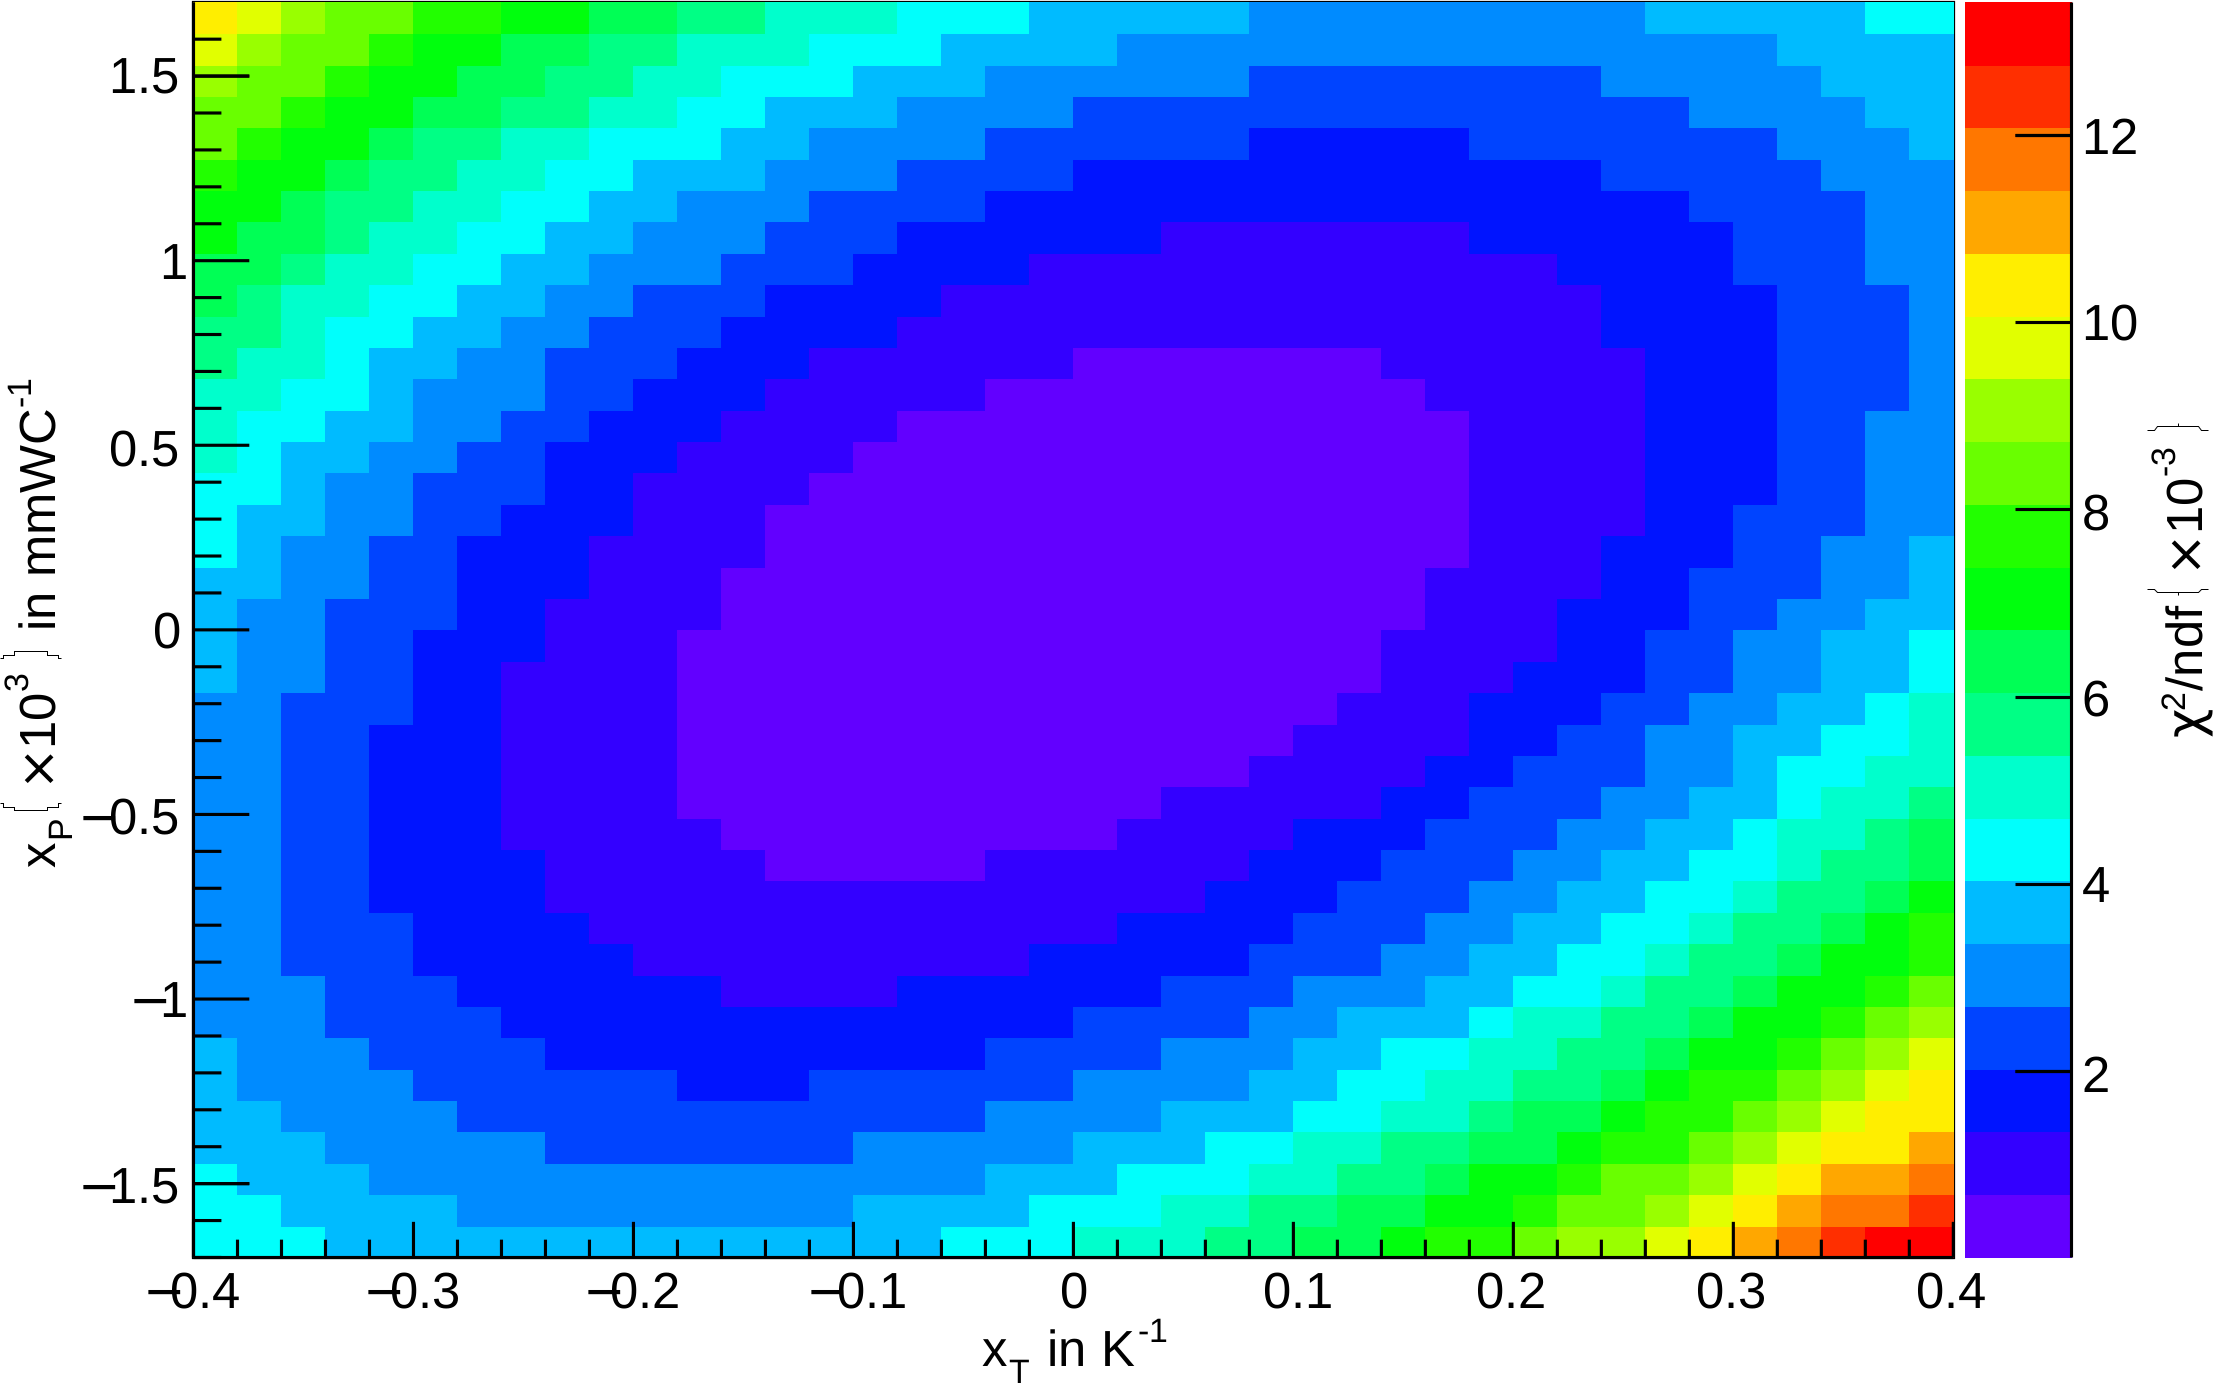
\includegraphics[width=0.8\textwidth]{cor_factors.png}
    \caption{$\chi^2/\textrm{ndf}$ values of the straight line fit for the
      plots of $\frac{\mathrm{d}n_{\textrm{rpc}}}{\mathrm{d}t}$ vs
      $\frac{P_{\textrm{rpc}}^{2}-P_{\textrm{atm}}^{2}}{2P_{\textrm{rpc}}}$ for different
      combinations of $x_T$ and $x_P$ for sample RPC gap-1.}
    \label{fig:xp}
  \end{figure}
\item In order to reduce the uncertainties at the minimum
  $\chi^2/\textrm{ndf}$, the procedures [\ref{itm:cor1}--\ref{itm:cor3}] are
  repeated for multiple iterations with subsequently smaller range of $x_T$
  and $x_P$ to obtain the final values.
\end{enumerate}

In the current case of sample RPC gap-1, the correction terms at minimum
$\chi^2/\textrm{ndf}$ are found to be
\[x_T=-3.23\times10^{-3}\textrm{\,K}^{-1}\textrm{ and }x_P=7.83\times10^{-5}\textrm{\,mmWC}^{-1}\textrm{.}\]

The negative value of the $x_T$ denotes that the volume of the gas-gap
increases with increase in room temperature and the positive value of the
$x_P$ denotes that the volume of the gap decreases with increase in atmospheric
pressure. In both cases, the values do not contradict with the Ideal Gas Law.
After including the best-fit values of $x_T$ and $x_P$ in the
equation~\ref{eq:ct}, the amount of gas inside the RPC gap
$\left(n_{\textrm{rpc}}\right)$ against time is shown in the Figure~\ref{fig:with}.
\begin{figure}[h]
  \centering
  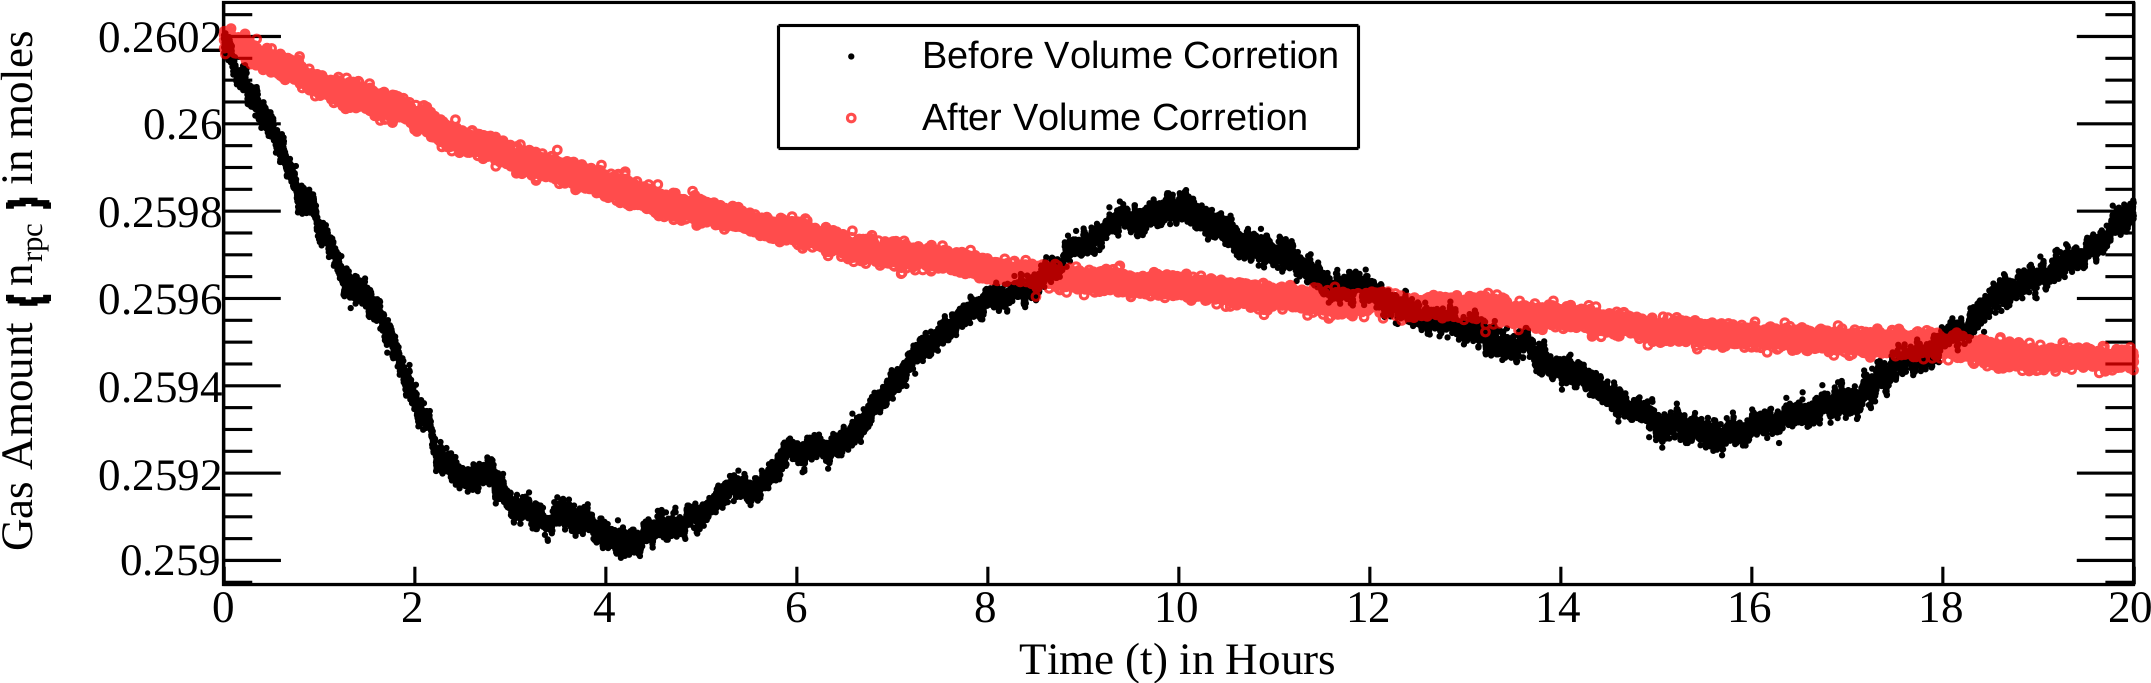
\includegraphics[width=0.99\textwidth]{M_t_57.png}
  \caption{Amount of gas in the RPC before (Black) and after (Red) correction
    for sample RPC gap-1.
  }
  \label{fig:with}
\end{figure} 
It can be noted in the Figure~\ref{fig:with} that the apparent
increase of gas amount seen earlier without the correction is resolved
after applying the volume correction. The effect of the volume
correction also can be observed in the plot of
$\frac{\mathrm{d}n_{\textrm{rpc}}}{\mathrm{d}t}$ vs
$\frac{P_{\textrm{rpc}}^{2}-P_{\textrm{atm}}^{2}}{2P_{\textrm{rpc}}}$ in the
Figure~\ref{fig:qt} which follows a nice straight line as expected
from Poiseuille's equation.
\begin{figure}[h]
  \centering
  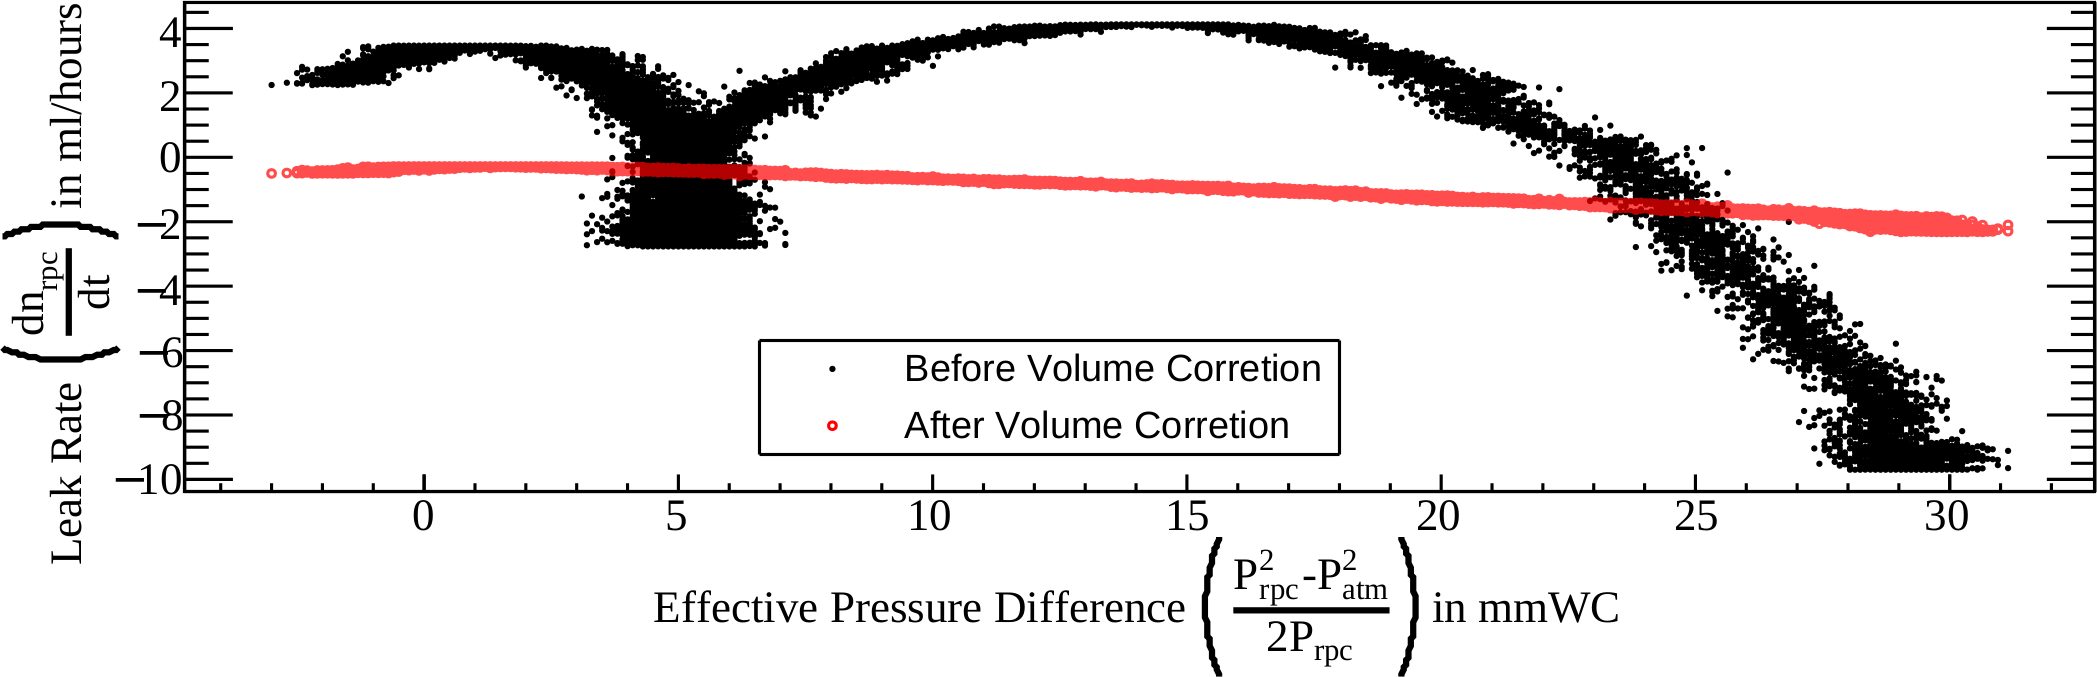
\includegraphics[width=0.99\textwidth]{Q_dP_57.png}
  \caption{$\frac{\mathrm{d}n_{\textrm{rpc}}}{\mathrm{d}t}$ vs
    $\frac{P_{\textrm{rpc}}^{2}-P_{\textrm{atm}}^{2}}{2P_{\textrm{rpc}}}$ plots before
    (Black) and after (Red) correction for sample RPC gap-1.}
  \label{fig:qt}
\end{figure}

The value of $\textrm{C}_{\textrm{Leak}}$ calculated from the
Figure~\ref{fig:qt} is
\[\textrm{C}_{\textrm{Leak}}=-\left(6.73\pm 0.007\left(\textrm{stat}\right)\right)\times 10^{-2}\textrm{\,ml\,hour$^{-1}$\,mmWC$^{-1}$}.\]

The negative value of $\textrm{C}_{\textrm{Leak}}$ implies that the
leakage of gas is from inside to outside, which again agrees with the
value of the pressure difference. Now, if this RPC gap is kept under a
constant pressure difference of 20\,mmWC, then it would leak a total
of 1.442\,$m$mol or 32.3\,ml gas in 24\,hours. This RPC gap thus can
be tagged as leaky.\footnote{The accepted value of the leak rate
  is greater than -0.02\,ml\,hour$^{-1}$\,mmWC$^{-1}$ and detailed are
  given in the section~\ref{sec:summary}.}

The Figure~\ref{fig:with1} and \ref{fig:qt1} show the test results for
another RPC gap (namely, gap-2).
\begin{figure}
  \centering
  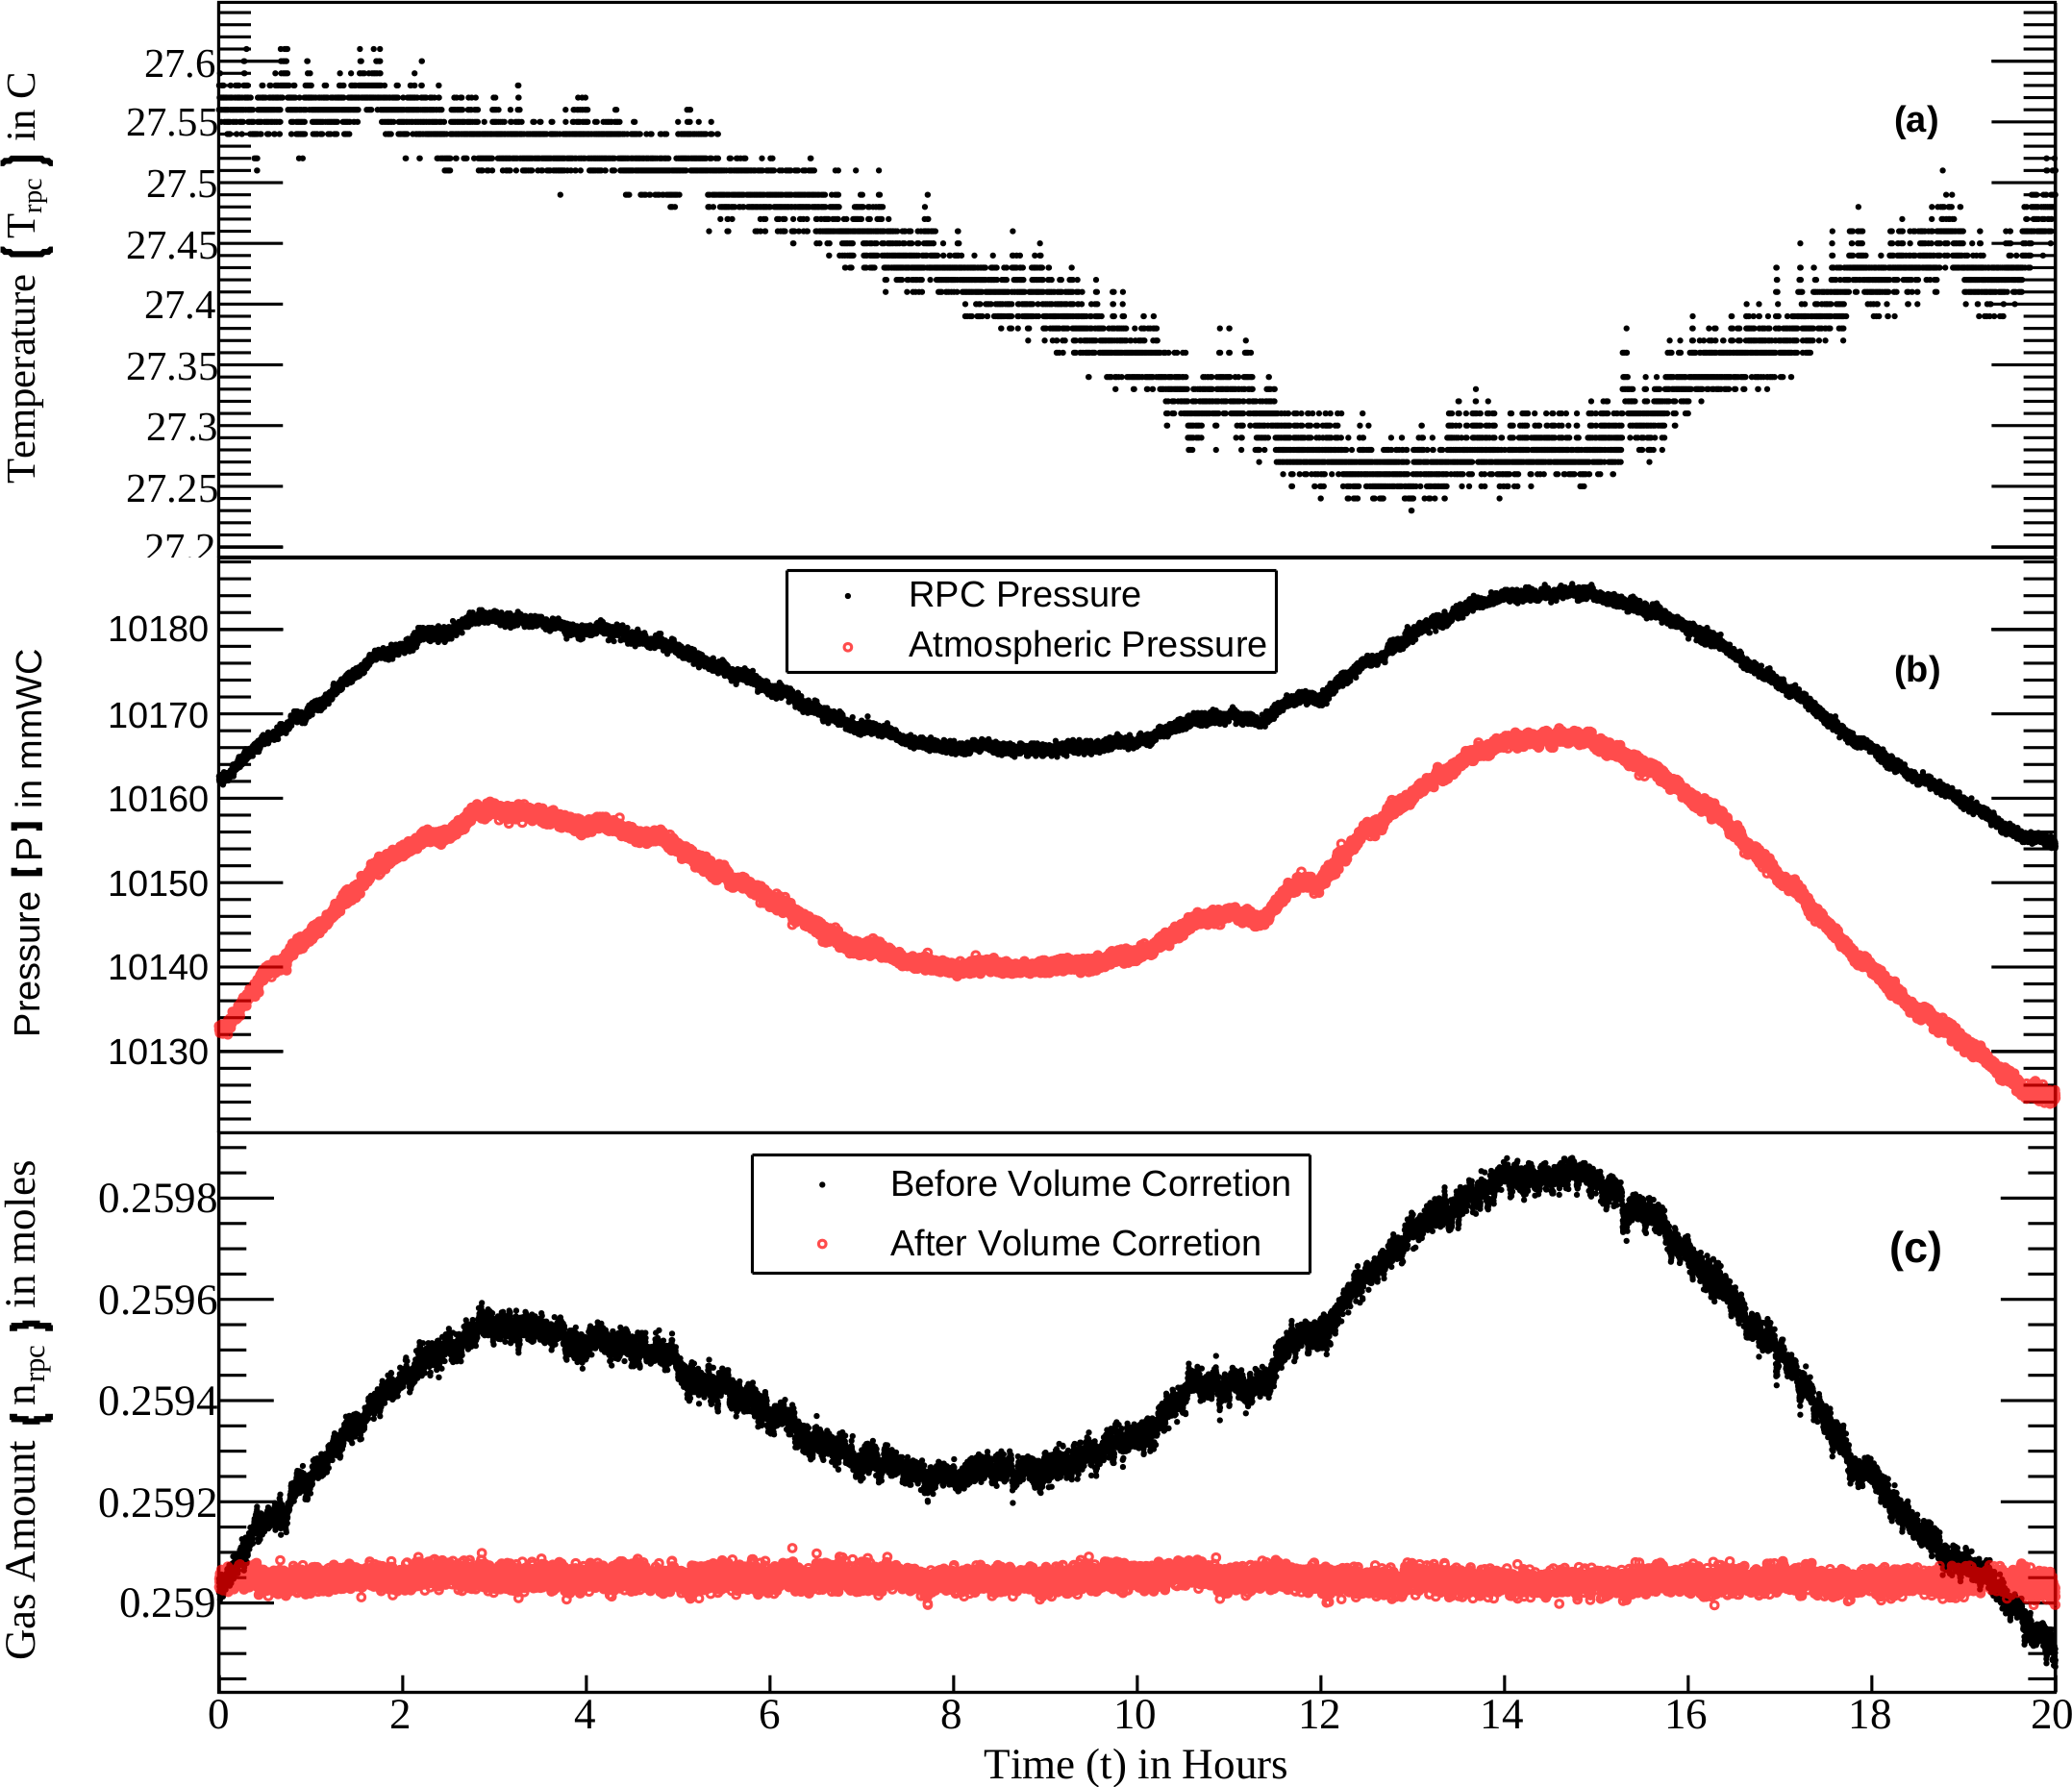
\includegraphics[width=0.99\textwidth]{all_130_gen.png}
  \caption{\textbf{(a)} Variation of temperature ($T_{\textrm{rpc}}$) with time,
    \textbf{(b)} Variation of atmospheric ($P_{\textrm{atm}}$ : Black) and RPC
    ($P_{\textrm{rpc}}$ : Red) pressure with time, \textbf{(c)} Amount of gas in
    the RPC before (Black) and after (Red) correction for sample RPC gap-2.}
  \label{fig:with1}
\end{figure}
\begin{figure}
  \centering
  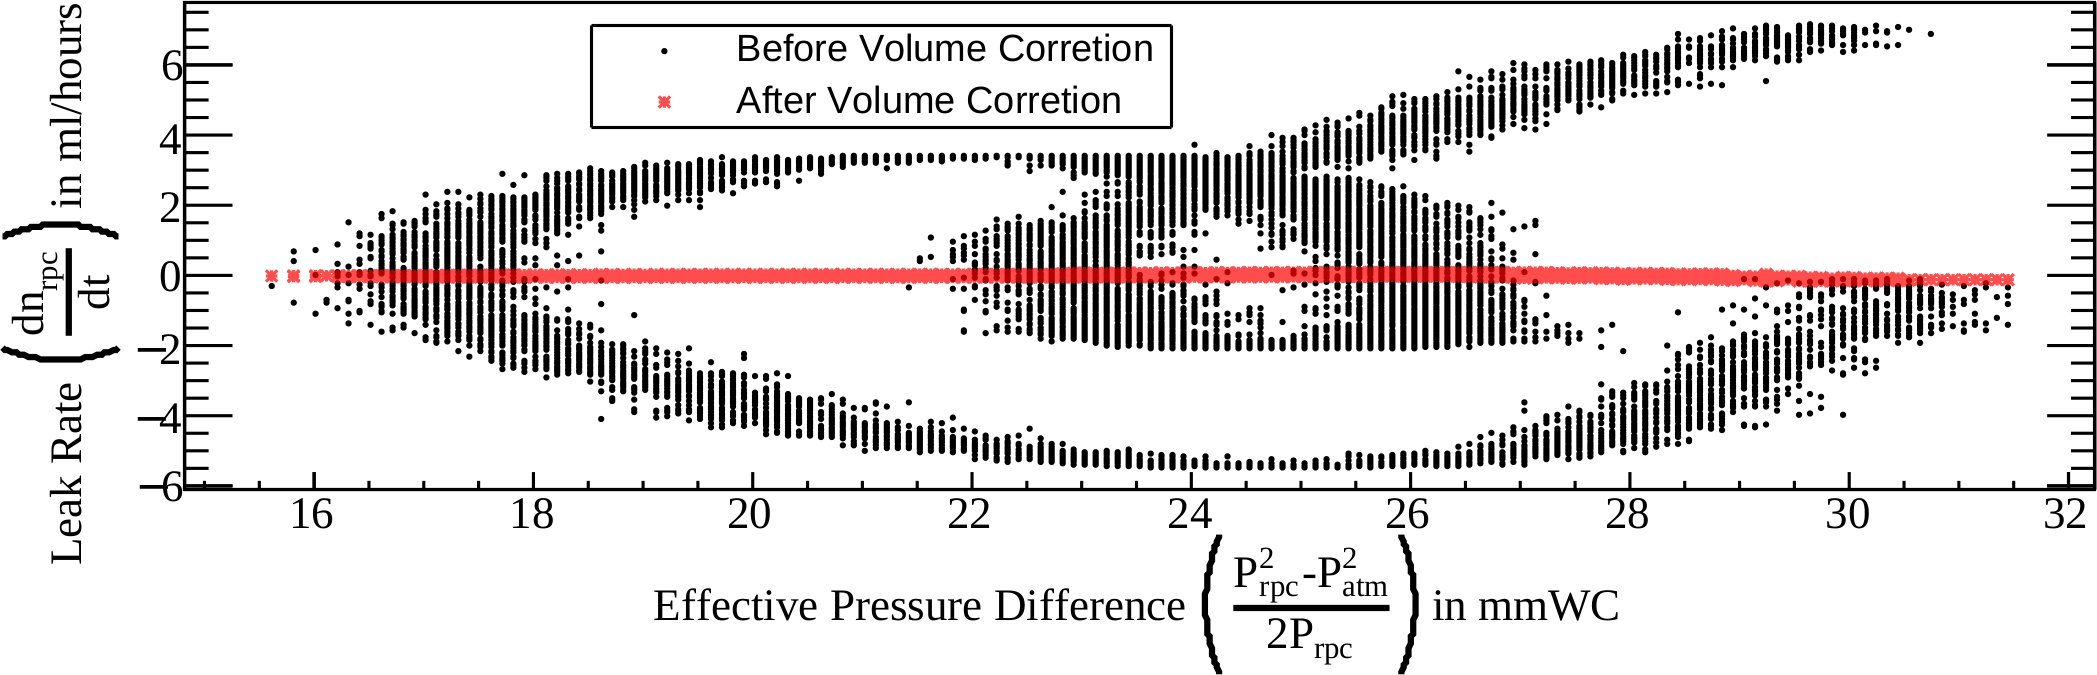
\includegraphics[width=0.99\textwidth]{Q_dP_130.png}
  \caption{$\frac{\mathrm{d}n_{\textrm{rpc}}}{\mathrm{d}t}$ vs
    $\frac{P_{\textrm{rpc}}^{2}-P_{\textrm{atm}}^{2}}{2P_{\textrm{rpc}}}$ plots
    before (Black) and after (Red) correction for sample RPC gap-2.}
  \label{fig:qt1}
\end{figure}
From the Figure~\ref{fig:qt1}, the value of $\textrm{C}_{\textrm{Leak}}$
for this RPC gap is estimated to be
\[\textrm{C}_{\textrm{Leak}}=-\left(5.1\pm 0.15\left(\textrm{stat}\right)\right)\times 10^{-4}\textrm{\,ml\,hour$^{-1}$\,mmWC$^{-1}$}.\]
In this case, the total leak would be 10.93\,$\mu$mol or 0.245\,ml of
gas within 24\,hours if a constant pressure difference of 20\,mmWC is
maintained.
The leak from this RPC gap is much smaller than the one discussed
earlier.

One of the aims of this study is to estimate the optimum (or minimum) time
required for calculating the leak rate satisfactorily. As seen in the
Figure~\ref{fig:temp}, the duration of the test is about 20\,hours. Several
calculations of the leak rate $\left(\textrm{C}_{\textrm{Leak}}\right)$ are
performed starting with the same data set, but up-to different lengths. In the
Figure~\ref{fig:time}, the value of $\textrm{C}_{\textrm{Leak}}$ for different
duration of data is plotted.
\begin{figure}
  \centering
  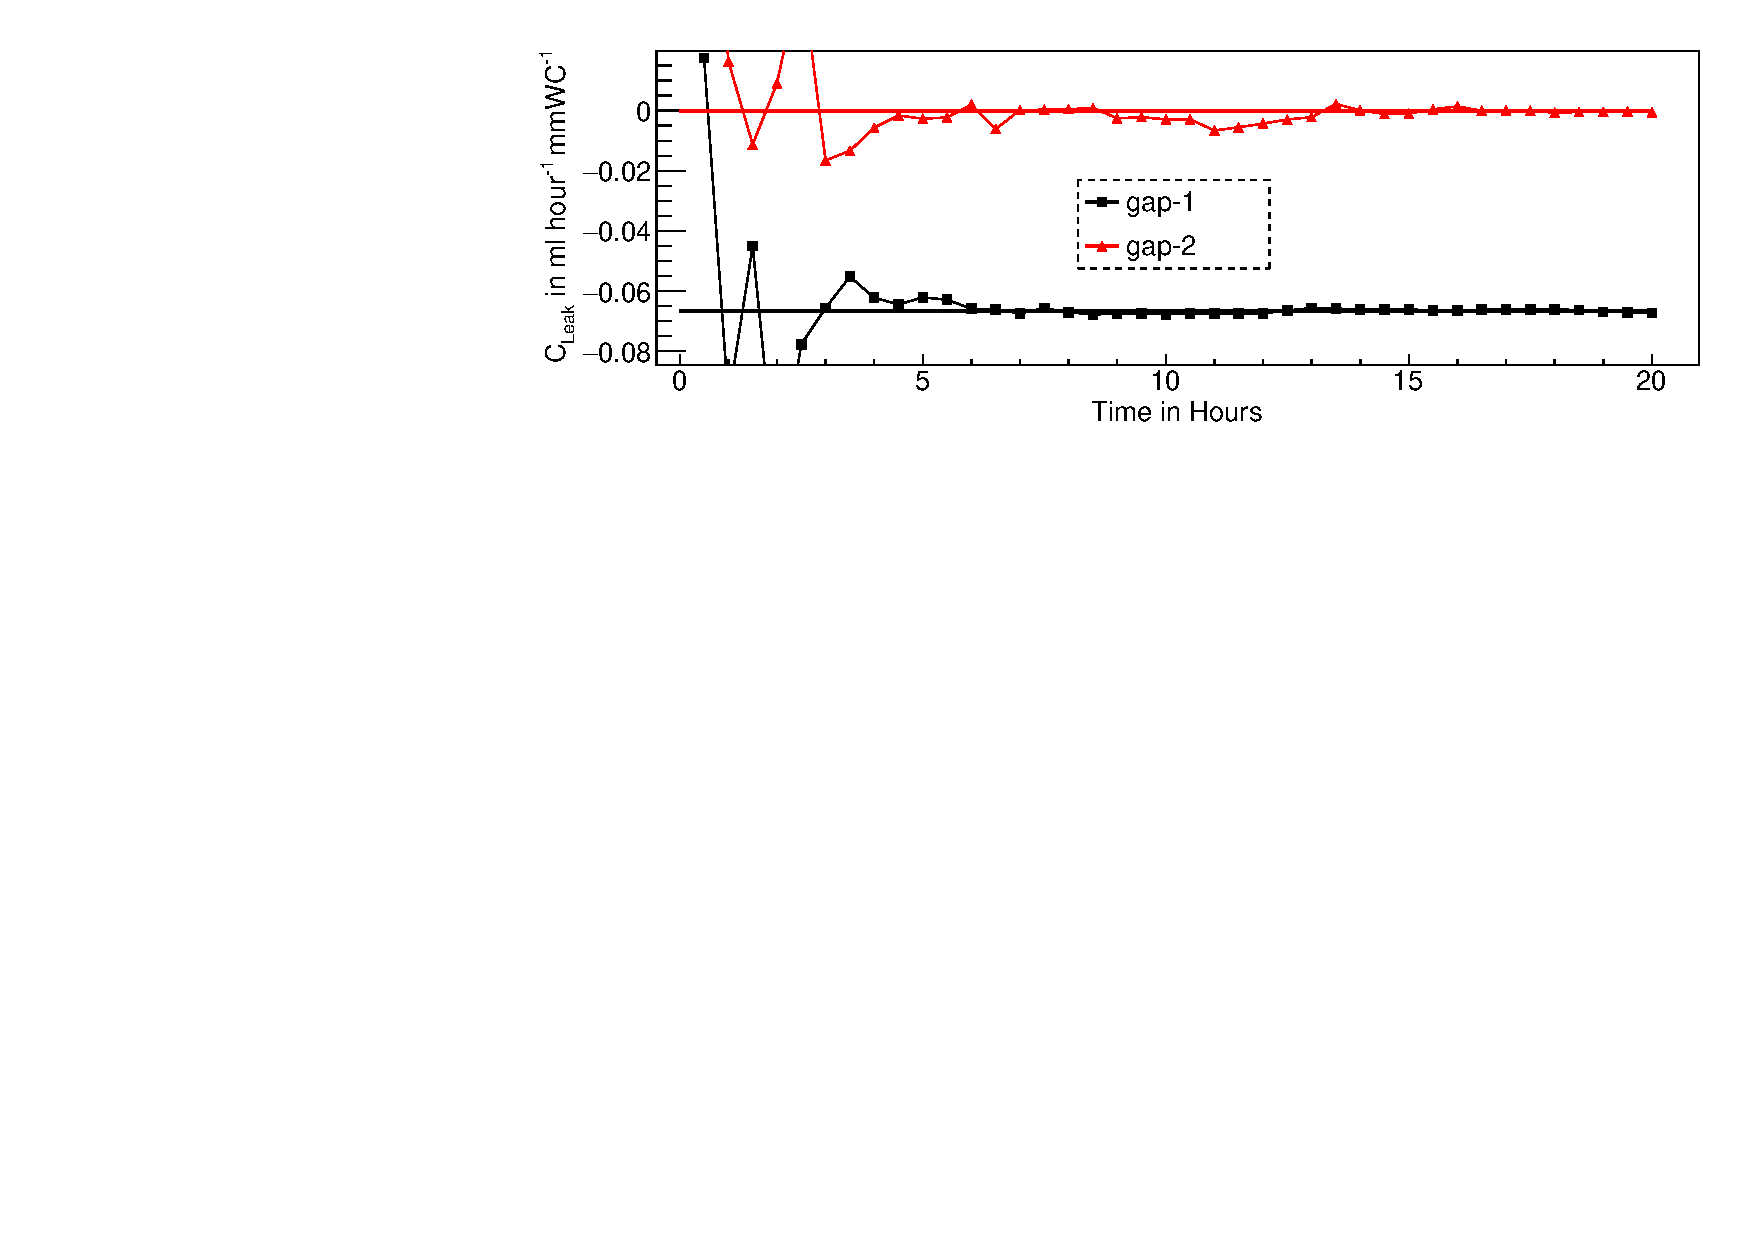
\includegraphics[width=0.99\textwidth]{conf_57_130.pdf}
  \caption{Leak rate estimation for data sets of different length for
    gap-1 and and gap-2.}
  \label{fig:time}
\end{figure}
For RPC gap-1, it can be observed that a minimum of 7-8 hours is
required to estimate the leakage without significant uncertainty. This
method requires a significant amount of data to fit the
$\frac{\mathrm{d}n_{\textrm{rpc}}}{\mathrm{d}t}$ vs
$\frac{P_{\textrm{rpc}}^{2}-P_{\textrm{atm}}^{2}}{2P_{\textrm{rpc}}}$ plots in
order to get proper results. Hence, the minimal time required for a
test will depend on the quantity of the leakage and also the
environmental conditions during the
test. If the leak rate is very small then more time is needed. In the
case of RPC gap-2, it can be observed from Figure~\ref{fig:time}
that about 7 hours is required to estimate leak rate with an
uncertainty of $\sim 2\times 10^{-3}$\,ml\,hour$^{-1}$\,mmWC$^{-1}$,
but about 15 hours is needed to have a result with uncertainty less
than $\sim 2\times 10^{-4}$\,ml\,hour$^{-1}$\,mmWC$^{-1}$.

It would also be noted that the calculation of $\textrm{C}_{\textrm{Leak}}$
directly depends on the value of $V_{\textrm{rpc}}$. The relative error in
measurement of $V_{\textrm{rpc}}$ will directly propagate to the relative
error in calculation of $\textrm{C}_{\textrm{Leak}}$.

\subsection{Systematic Error}
A well defined method should be able to reproduce the same result in a
repeated test under different test conditions.
The success of this procedure depends on the periodic changes of
ambient pressure and temperature which are largly unpredictable.
To estimate the systematic error in the estimation of
$\textrm{C}_{\textrm{Leak}}$, one of the RPC gaps is tested for 48 hours.
Several data samples of equal duration have been generated from this
large data sample and `$\textrm{C}_{\textrm{Leak}}$'s are estimated in
each case. The Figure~\ref{fig:systematic}(a) shows the distribution
of the estimated `$\textrm{C}_{\textrm{Leak}}$'s for data samples of the
duration of 25 hours.
\begin{figure}
  \centering
  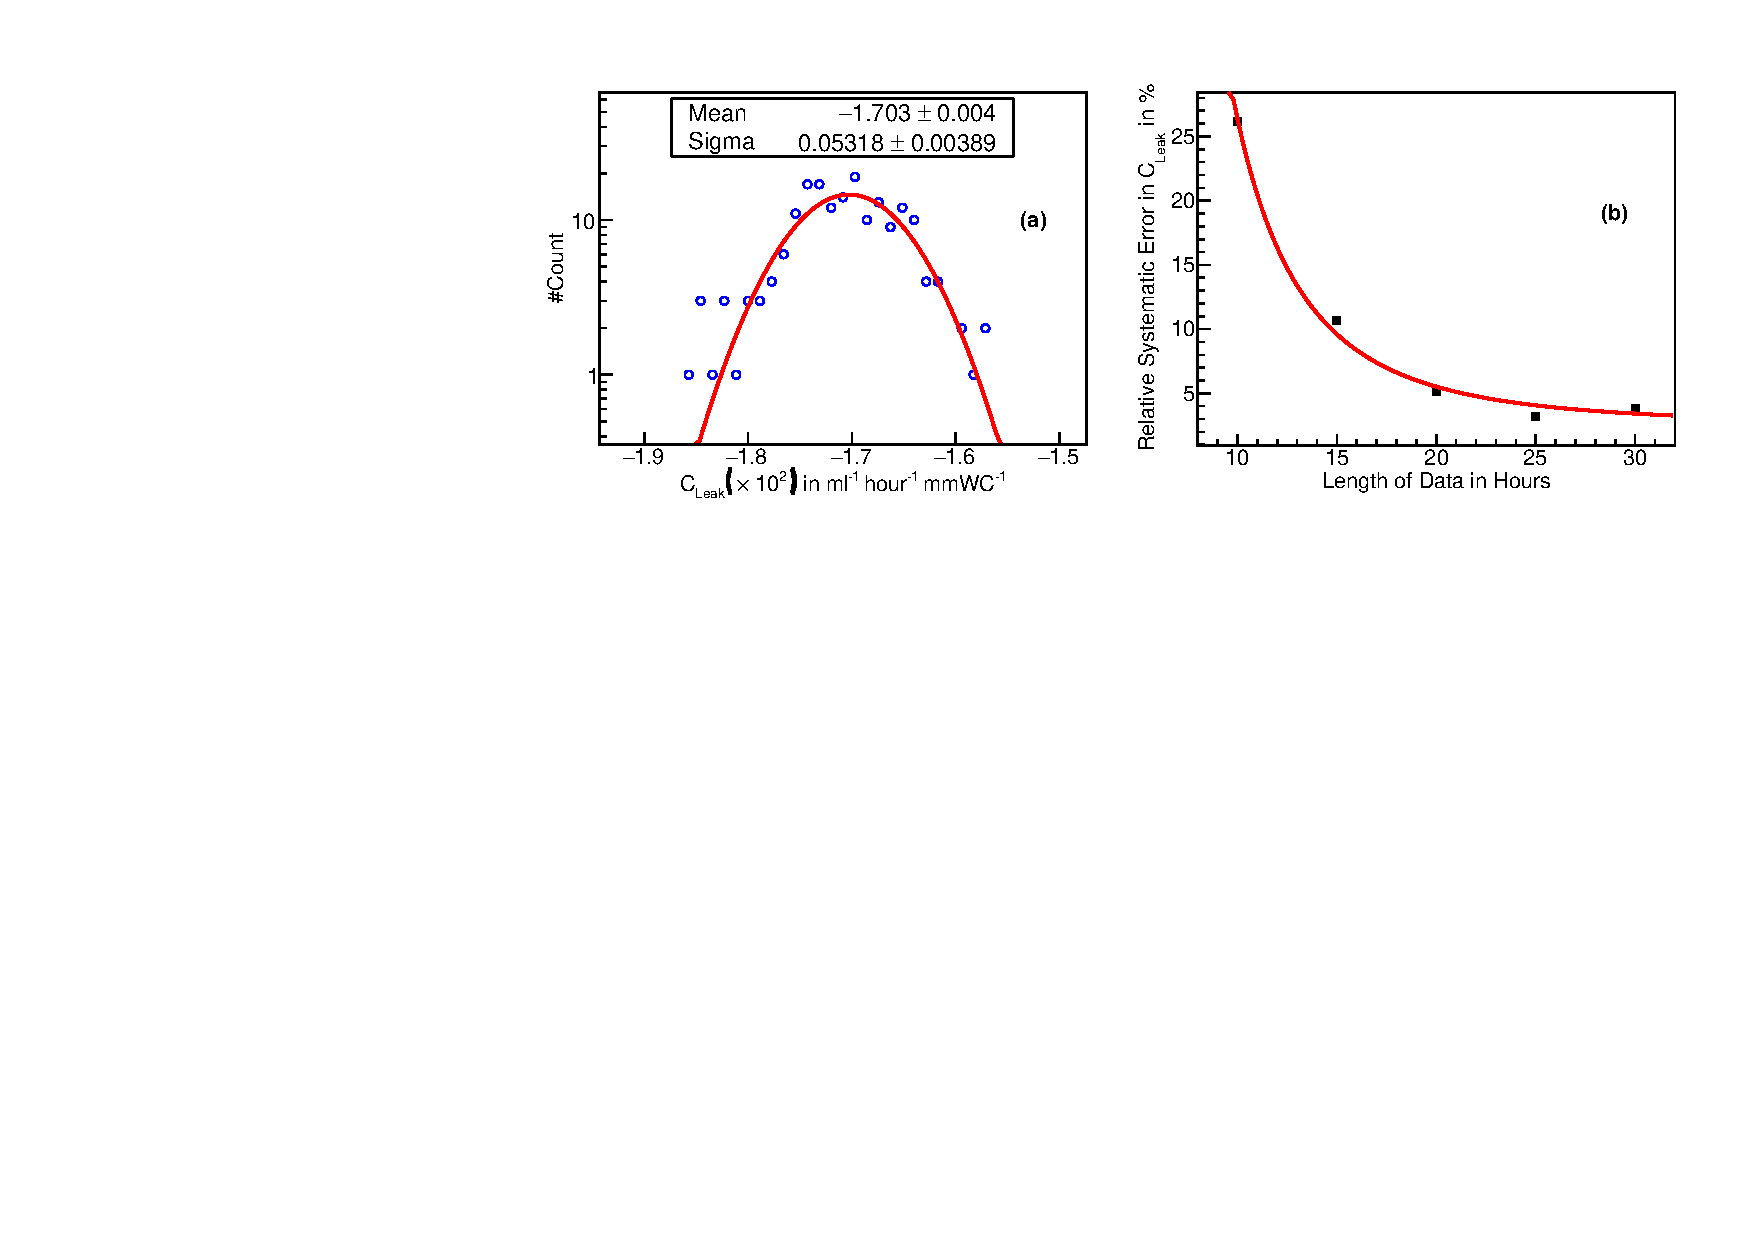
\includegraphics[width=0.99\textwidth]{splitDataLeak.pdf}
  \caption{\textbf{(a)} Systematic error with data sets with length of
    25 hours, \textbf{(b)} Variation of relative systematic error with
    length of data.}
  \label{fig:systematic}
\end{figure}
The relative width of $\textrm{C}_{\text{Leak}}$ for the different
duration of time is presented in Figure~\ref{fig:systematic}(b),
which is considered a systematic error of this measurement. For a
longer duration it is about 3.1\%.
As expected, it can be observed that by lengthening the test duration,
the relative systematic uncertainty in the measurement of
$\textrm{C}_{\textrm{Leak}}$ decreases significantly.

\subsection{Result of the Tested RPC Gaps}
The set-up and the procedures described in this chapter have been
used to test eighty RPC gaps. The results of these tests are
summarised in the Figure~\ref{fig:conclusion}
\begin{figure}[h]
  %% \vspace*{-15pt}
  \centering
  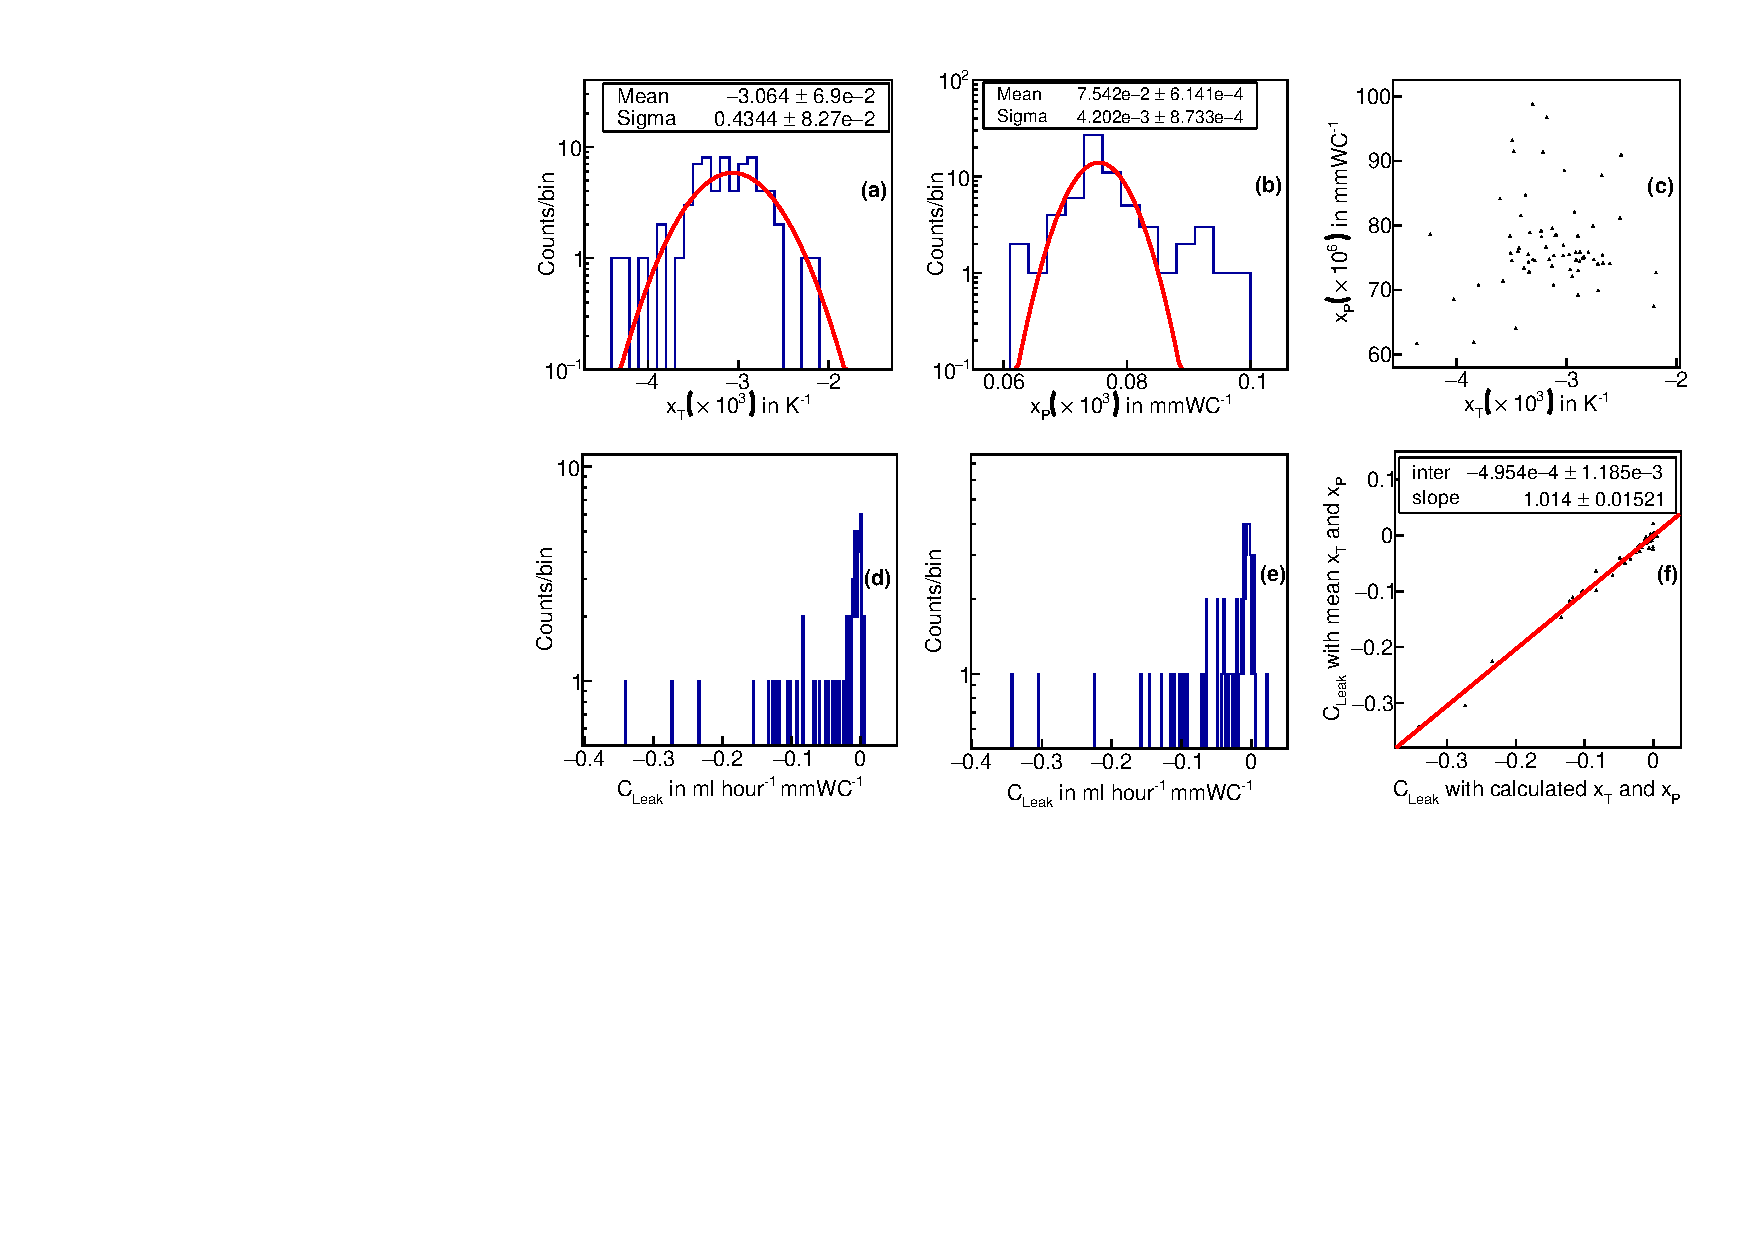
\includegraphics[width=0.99\textwidth]{Leak_Conclusion.pdf}
  \caption{\textbf{(a)} $x_T$ values of eighty RPC gaps,
    \textbf{(b)} $x_P$ values of eighty RPC gaps,
    \textbf{(c)} Correlation between minimised values of $x_T$ and $x_P$
    for eighty RPC gaps,
    \textbf{(d)} $\textrm{C}_{\textrm{Leak}}$ of eighty RPC gaps with calculated
    values of $x_T$ and $x_P$,
    \textbf{(e)} $\textrm{C}_{\textrm{Leak}}$ of eighty RPC gaps with mean
    values of $x_T$ and $x_P$,
    \textbf{(f)} Correlation between $\textrm{C}_{\textrm{Leak}}$ obtained by
    both calculated and mean values of $x_T$ and $x_P$ for eighty RPC gaps.}
  \label{fig:conclusion}
\end{figure}
and general findings are listed here.
\begin{itemize} \itemsep -3pt
\item The correction parameters depend on the structure of each of the
  RPC gaps. The values of $x_T$ and $x_P$ should ideally be the same
  for similar type of RPC gaps, but it is almost impossible to
  manufacture inch-perfect replicas. Any gap with popped up button
  spacers(s) (`button pop-up' is discussed in Section~\ref{sec:button})
  will also reflect higher values of these two parameters. This causes
  the spread in the values of $x_T$ and $x_P$ which can be seen in
  the Figure~\ref{fig:conclusion}(a) and \ref{fig:conclusion}(b),
  respectively.
\item The minimised values of $x_T$ and $x_P$ for a gas gap are two independent
  parameters. As expected, it can be seen in the Figure~\ref{fig:conclusion}(c)
  that there is no correlation between these two parameters for eighty RPC gaps
  which were tested.
\item The Figure~\ref{fig:conclusion}(d) shows the values of
  $\textrm{C}_{\textrm{Leak}}$ for eighty RPC gaps where the values of $x_T$ and
  $x_P$ are calculated explicitly for each RPC gap. The
  Figure~\ref{fig:conclusion}(e) shows the same but with the mean values of
  $x_T$ and $x_P$ obtained from \ref{fig:conclusion}(a) and
  \ref{fig:conclusion}(b), respectively.
\item Figure~\ref{fig:conclusion}(f) shows correlation between
  $\textrm{C}_{\textrm{Leak}}$ obtained by calculated $x_T$ and $x_P$ values
  explicitly for each chamber (shown in the Figure~\ref{fig:conclusion}(d))
  and by mean $x_T$ and $x_P$ values (shown in the
  Figure~\ref{fig:conclusion}(e)). The nature of correlation is direct.
  So, mean values of $x_T$ and $x_P$ can also be used for a quick calculation
  saving CPU time.
\end{itemize}

\section{Chapter Summary}\label{sec:summary}
The method outlined above can give a quantitative estimation of the
leak of an RPC with higher precision and in much less time compared to
what may be obtained using a conventional manometer. This method can
be used for any kind of sealed chambers other than RPC where the
structure of the chamber is prone to deform due to variation in
ambient pressure and temperature. As discussed in the reference
\cite{rpcleak2016}, it is possible to eliminate the effect caused by
ambient temperature by the use of an enclosure where the temperature
is controlled precisely in case of abrupt and/or irregular changes in
ambient temperature, causing difficulties in the calculation of volume
correction factors. It should be noted that the minimum time required
for a test will depend on extent of the leakage. If the leak rate is
very small then more time is needed, but most of the gaps were
possible to be tested within 7-8 hours with an accuracy of
$\sim 2\times 10^{-3}$\,ml\,hour$^{-1}$\,mmWC$^{-1}$. Currently, a gas
gap is considered as usable if its $\textrm{C}_{\textrm{Leak}}$ value is
greater than $-0.02$\,ml\,hour$^{-1}$\,mmWC$^{-1}$. If the RPCs are
operated at an excess pressure of 10\,mmWC above atmospheric pressure,
the total leakage from ICAL detector will be approximately
6\,litres/hour during its active operation.

The leak-test setups, both wired and wireless, are built and tested.
The setups are now being used at various facilities and industries
working along with INO-Collaboration. With the help of the prepared
document, even a novice can test a large number of RPCs in a short
time. The difficulty in handling a glass RPC increases significantly
with its size. As the present method does not require the RPC to be
moved during the tests. Also, the
knowledge gained in this study gives us more opportunity to better
understand the structural integrity of the glass RPCs against various
atmospheric parameters.

The work presented in this chapter is published in \cite{rpcleak}.
